\section{Type II Weyl semimetals}

The conic section problem with the intersecting plane restricted to pass through the node of the cone is trivially seen to have two solutions: a point and two intersecting lines.
Despite this, the possibility of a Weyl cone tilted beyond the Fermi level was never considered before \citeauthor{soluyanovTypeIIWeylSemimetals2015} described this new class of Weyl semimetals in 2015.
This now seemingly obvious possibility made an already rich field even more exciting, opening up for a wider range of novel and interesting effects.
\todo{add some concrete examples or cites}

In the case of massless fermions, the particle physics equivalent of the Weyl semimetal, such a tilt is not possible, due to the requirement of Lorentz invariance \todo{add cite or explain}.
In condensed matter physics, however, this is not an issue, and it is indeed a real class of materials \todo{cite examples}.
We denote these types of materials Type-II Weyl semimetals, as opposed to Type-I.
The transition between Type-I and Type-II is abrubt -- the Fermi surface goes form a single point to two intersecting lines, in other words going from a zero dimensional to a one dimensional surface.
\todo{Make sure this is indeed a one dimensional surface. It is kind of 1DxZ(2)}
\todo{Make sure it is one dim also for the 3D case, quadric surface, not conic intersection}
Type-II also has electron and particle pockets at the Fermi level.
While the density of states for a Type-I semimetal goes to zero as one approaches the Fermi level, this causes Type-II to have a finite density of states at the Fermi level.
\todo{End with something like: all in all this gives type ii weyl semimetal manifestly different properties from tyep i, useful both in practical applications and as an interesting phenomena seen from a purely scientific perspective}

\subsection{Hamiltonian}
We will firstly consider a slightly more realistic toy model for a Weyl semimetal, with a parameter taking the system from a Type-I to a Type-II.
This is instructive both in order to more intuitively see the origin of the terms causing the tilting of the Dirac cone, and also to see how two Dirac cones in the same Brillouin zone tilt in relation to each other.
We will then continue by linearizing the model around the Weyl points, regaining the familiar form of a Dirac cone, with an additional anisotropy term causing the tilt.

Using the general time-reversal breaking model described by \citeauthor{mccormickMinimalModelsTopological2017} we have
\begin{equation}
  \begin{split}
    H(\vec{k}) &= \left[ ( \cos k_x + \cos k_z - 2 )m + 2 t (\cos k_x - \cos k_0) \right] \sigma_1\\
    &\pe - 2 t \sin k_y \sigma_2 - 2t \sin k_z \sigma_3
    + \gamma (\cos k_x - \cos k_0).
  \end{split}
\end{equation}
The model has Weyl nodes at \(\vec{K}' = (\pm k_{0}, 0,0)\), and the parameter $\gamma$ controls the tilting of the emerging cones.
A value of $\gamma=0$ gives no tilt, while for $\gamma > |2 t|$ the Type-II system emerges.
Figure \ref{fig:ridgeline} shows the cross section \(k_{y} = 0\) of the eigenvalues of this system, as \(\gamma\) is gradually increased from 0 to 0.15 \todo{verify numbers}.
The \(\gamma\)-term ``warps'' the bands, and in the limit of Type-II the hole band crosses the Fermi level into positive energy, while the particle band crosses the Fermi level into negative energies.
We call these hole and electron pockets, respectively.

Linearizing around the Weyl nodes reduces to the familiar expression of a Dirac cone
\begin{equation}
  \label{eq:37}
  H(\vec{K} ^{'\pm} + \vec{k}) \approx \mp 2 t k_{x} \sin k_{0} \sigma_{1} - 2 t (k_{y} \sigma_{2} + k_{z} \sigma_{3}) \mp \gamma k_{x} \sin k_{0} \sigma_{0}, \quad k_{x}, k_{y}, k_{z} \ll 1.
\end{equation}
When the separation between the two nodes is \(\pi\), i.e. \(k_{0} = \pi/ 2 \), the linearized Hamiltonian of around the cone, is
\begin{equation}
  \label{eq:38}
  H'(\vec{k}) = \mp 2 t k_{x} \sigma_{x} - 2t k_{y} \sigma_{y} - 2 t k_{z} \sigma_{z} \mp \gamma k_{x}.
  % h'(\vec{v}) = -2t \vec{k} \vec{\sigma} - \gamma k_{x}.
\end{equation}
However, as the two noes are brought closer together, the effective Fermi velocity in the \(x\)-direction is rescaled, and the system is anisotropic even for no tilt (\(\gamma=0\)).
The expression may be made even more clear by moving the sign \(\pm\)-sign into the tilt parameter \(\gamma\).
The Hamiltonian is invariant under a sign change of the first term, as the isotropic Dirac Hamiltonian is invariant under inversion.
In the tilt-term, we move the sign dependence into \(\gamma \), and the linearized model is
\begin{equation}
  \label{eq:39}
  H'(\vec{k}) = - 2t \vec{k} \vec{\sigma} - \gamma^{\pm} k_{x},
\end{equation}
where \(\gamma ^{\pm} = \pm \gamma \) with the upper sign corresponding to the node at \(k_{x} = + k_{0}\) and the lower sign corresponds to the node at \(k_{x} = - k_{0}\).
As expected, we get two Dirac cones, tilting in opposite direction, but with the same amount.
\todo{How does this affect the Berry curvature and chern number?}
\todo{Maybe prettier/more correct to invert ky and kz, as that would also give the opposite chirality of the dirac points}

The linearized model are accurate in describing low energy interactions around the Fermi level.
For higher energies their validity falls apart, and more complex models are warranted.
In our calculations the linear models is sufficient, and much easier to work with, and we will thus mainly consider the linear model from here on.

\begin{itemize}
  \item gives rise to cones tilting opposite direction
  \item Linearized model valid for low energy interaction. For higher energy, the perfect cone model is not valid, as the cones does in fact touch.
  \item In this model, the hole pocket is ``shared'' between the two cones. There are also models with individual pockets (see \cite{mccormickMinimalModelsTopological2017})
\end{itemize}

\begin{figure}[ht]
  \centering
  
\includegraphics[width=0.4\textwidth]{figures/conicSection}
  \caption{\label{fig:conic-section-sketch} }
\end{figure}


\begin{figure}[ht]
  \centering
  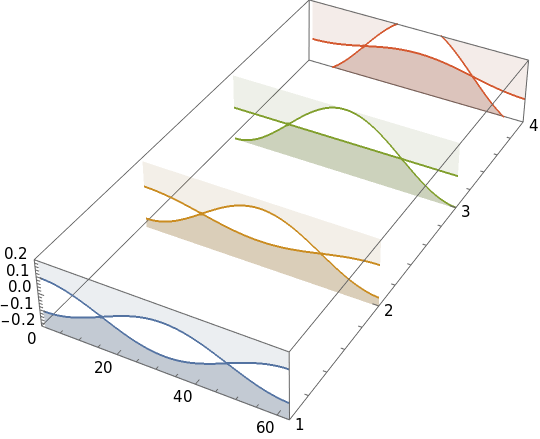
\includegraphics[width=0.7\textwidth]{figures/typeIIridgeline}
  \caption{\label{fig:ridgeline} \todo{Write this} The values of the parameters were chosen to be \(m=0.15, t=-0.05, \) and \(2 k_{0}=\pi\).}
\end{figure}

\begin{figure}[ht]
  \centering
  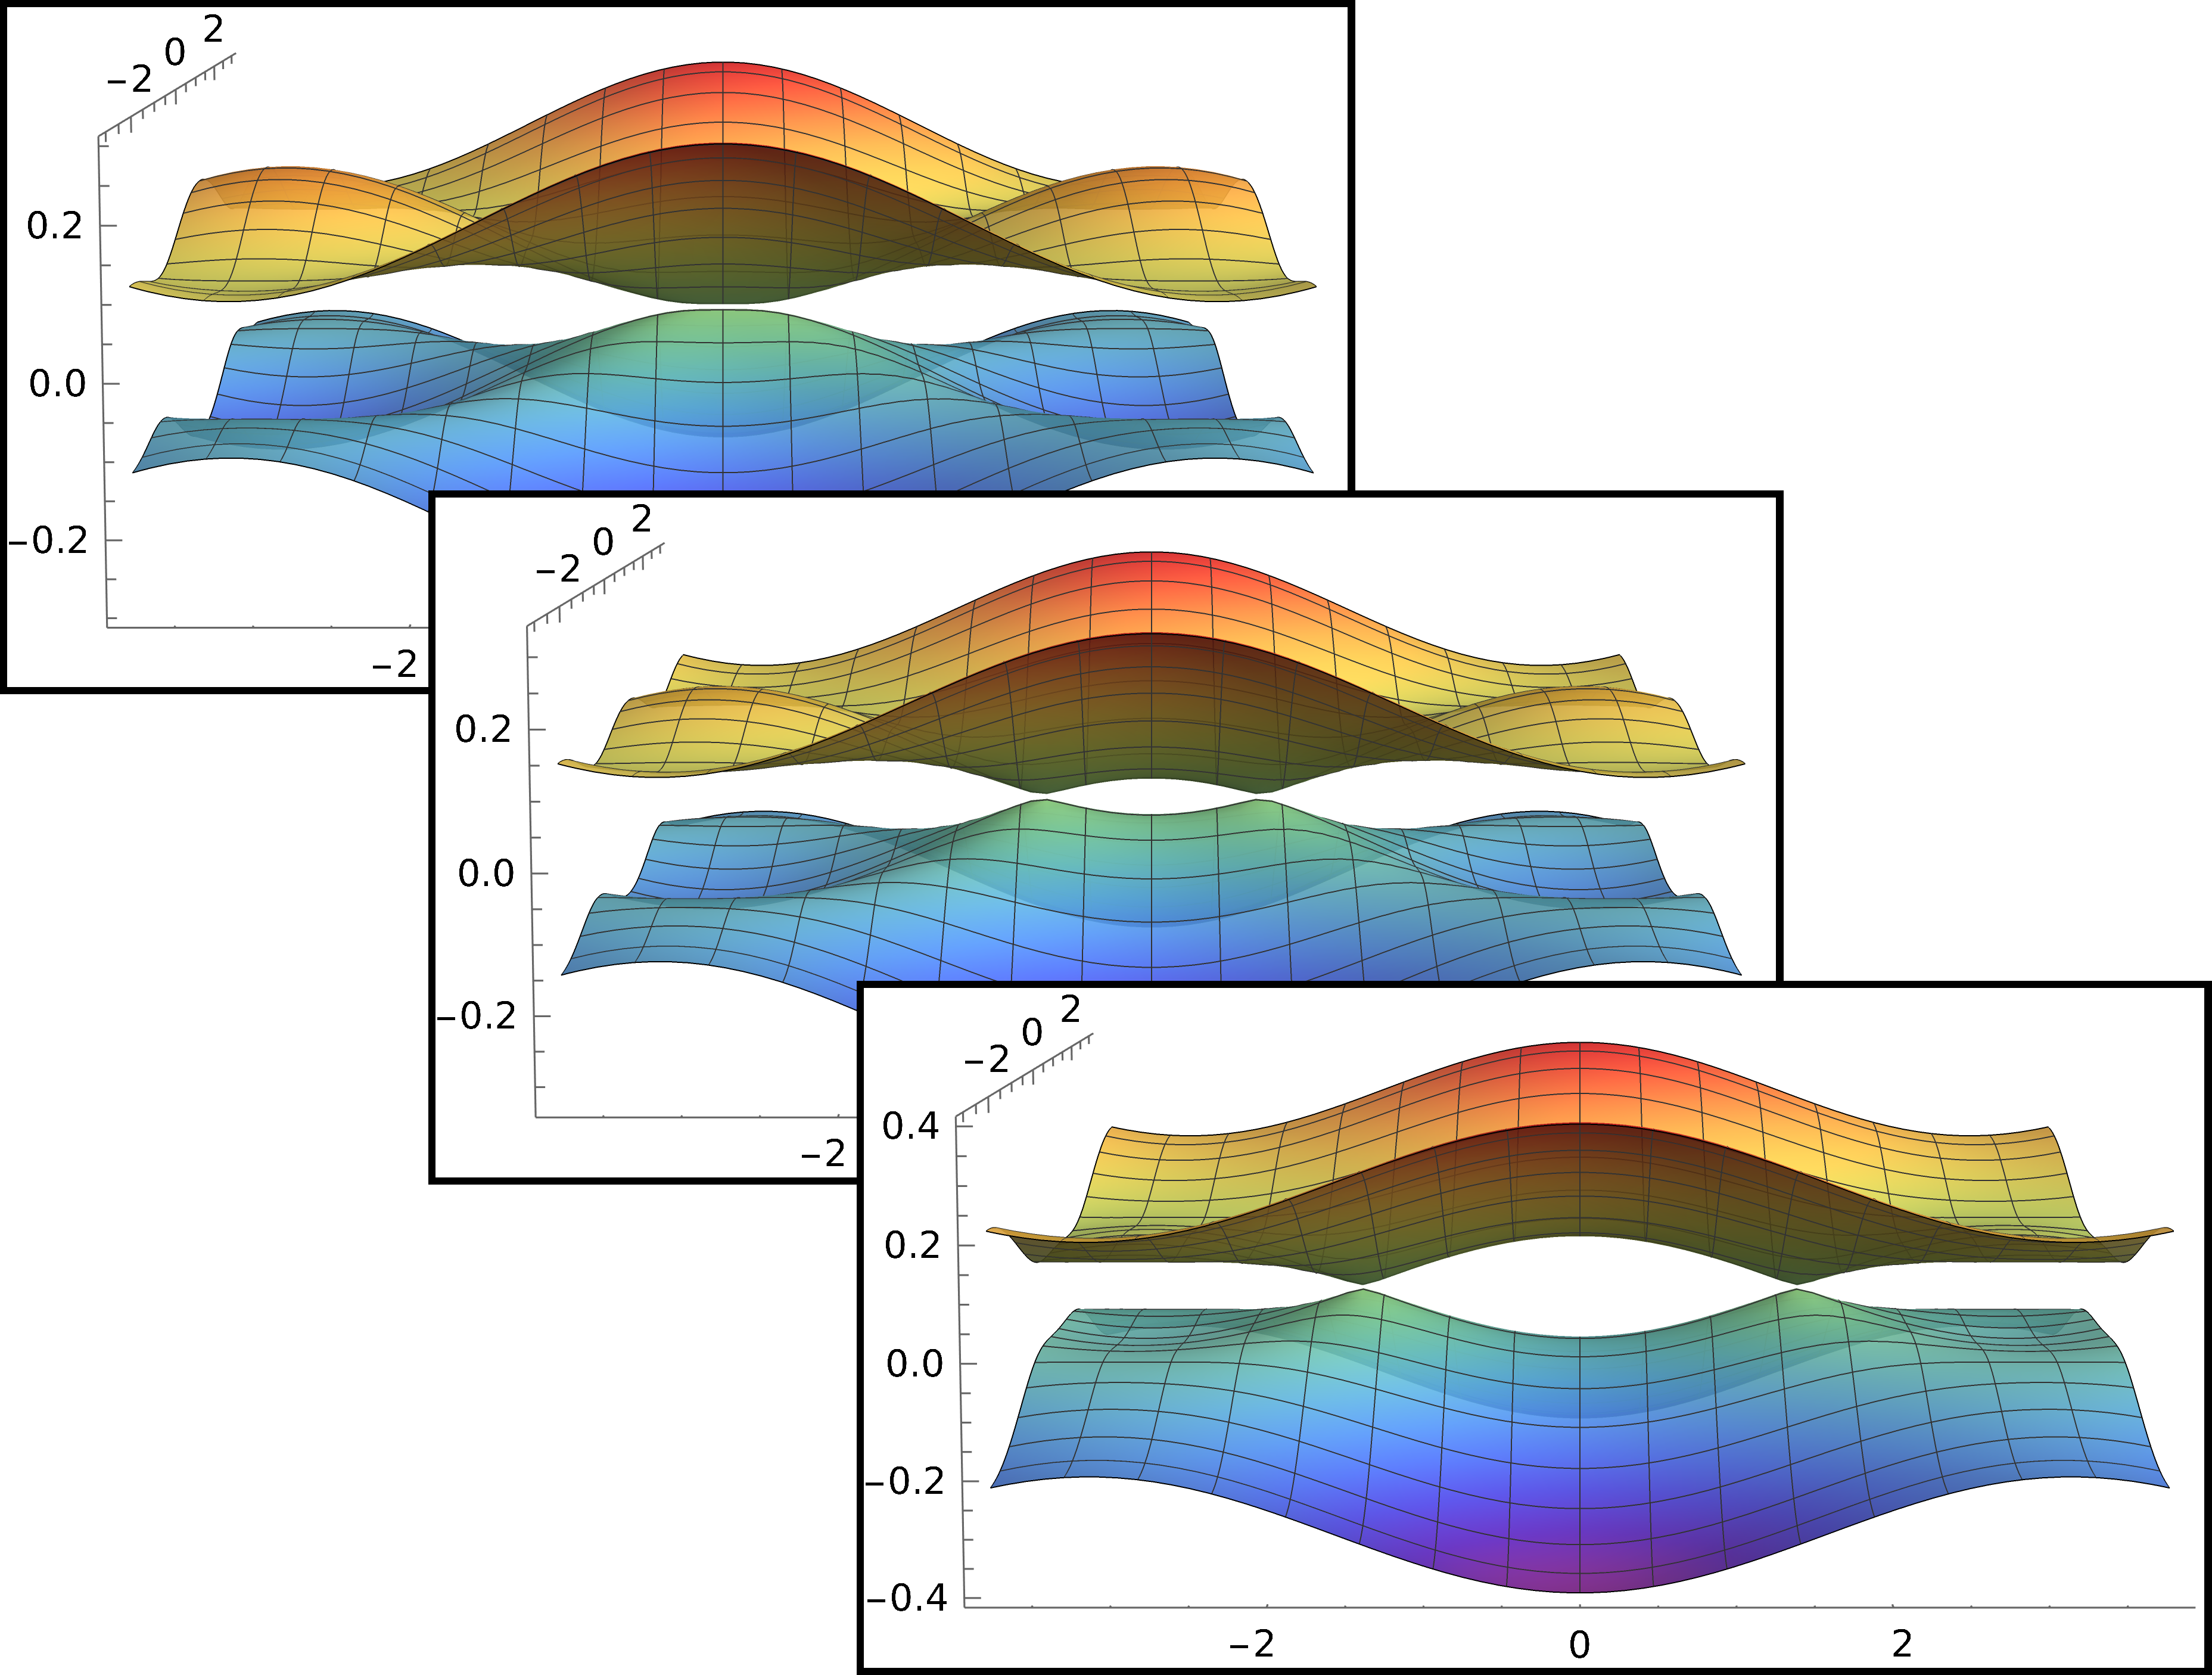
\includegraphics[width=0.7\textwidth]{figures/movetypeiinode}
  \caption{\label{fig:typeii:move-nodes} A Type-II Weyl semimetal with separation between the nodes \(2k_{0} = 0, \pi/2, \pi \).
    See main text for details about the model.}
\end{figure}


\subsection{Eigenstates and Landau levels}
The eigenvalues of Type-II Weyl semimetal are simple to find, and are not qualitatively different from those of Type-I, other than the appearance of particle and hole pockets at the Fermi level.
We will also consider the Landau levels of these materials, which importantly are very different from Type-I.
In fact, erroneous treatment of the Landau spectrum of Type-II semimetals caused the original paper describing Type-II materials to mistakenly assert that the chiral anomaly would not be present for certain directions of a background magnetic field \cite{soluyanovTypeIIWeylSemimetals2015}\cite{sharmaChiralAnomalyLongitudinal2017}.

Eigenstates, spin, berry, etc

The issue with the Landau level description is that for certain directions of the \(B\)-field, the Landau levels break down.
For Type-I materials, the description is valid for all directions of the \(B\)-field, but as the cone tip into a Type-II material, the description breaks down when the \(B\)-field and tilt direction are perpendicular \cite{sharmaChiralAnomalyLongitudinal2017}, and as the magnitude of the tilt increases, the Landau levels are only valid up to a certain angle between the tilt direction and magnetic field.
We will in this section derive and elucidate the Landau levels and their regions of validity.

Consider the Hamiltonian
\begin{equation}
  \label{eq:40}
  H = v_{F} \vec{t} \vec{k} + s v_{F} \vec{k} \vec{\sigma},
\end{equation}
where \(\vec{t}\) is the \emph{tilt vector} and \( v_F \) is the Fermi velocity
\footnote{In general, the Fermi velocity may be anisotropic, in which case the momentum enter as \( v_i k_i \), instead of \( v_F k_i \). By a rescaling of the momenta, we may consider any, in general anisotropic, system to be isotropic in velocity.}.
To find the Landau levels in a magnetic field \(\vec{B} = B_{z}\hat{z} \), we will ``Lorentz boost'' the system to a frame where the cone is not tilted, where we may use the usual approach for finding the Landau levels.
Firstly, assume that the tilt vector \(\vec{ t }\) is in the \(x,z\)-plane, \(\vec{t} = (t_{\perp}, 0, t_{\parallel})\), which we can always achieve by a rotation around \(z\).
\todo{Proof by figure}
Introduce the \(\vec{B}\)-field by the minimal coupling \(\vec{k} \to \vec{k}^B = \vec{k} + e \vec{A}\).
We take the field to be in the \( z \)-direction, and use the Landau gague \(\vec{A} = -B_{z}y \hat{x}\).

The Landau level equation is
\begin{equation}
  \label{eq:42}
  \left(H_{B} - E\right) \ket{\psi } = 0,
\end{equation}
with
\begin{equation}
  \label{eq:44}
  H_{B} = v_F \left(t _{\perp} k^B_{x} + t _{\parallel} k^B_{z} \right) \mathcal{I}_2 + \sum_i s v_{F} k^B_{i} \sigma _{i},
\end{equation}
where \(\mathcal{I}_{2}\) is the identity matrix of size 2.
In order to use the ladder operator method used for the untilted cone, we must get rid of the \(k^B_{x}\) on the diagonal of the Hamiltonian.
\footnote{It would also be possible to choose the frame such that the tilt was both in \(x\) and \(y\) direction, in which case we would get ladder operators also on the diagonal.
  This system, albeight tedious, could also have been solved directly.
  \todo{Verify this}
}
To achieve this, we will use a ``Lorentz transformation'', which as we will show only leave \(k_{z}\) and \(E\) in the diagonal.
Act with the hyperbolic rotation operator \(R = \exp[\Theta /2 \sigma_{x}]\) on Eq. \eqref{eq:42}, and insert identity on the form \(\exp[\Theta /2 \sigma_{x}]\exp[-\Theta /2 \sigma_{x}]\) before the state vector.
By introducing the state in the rotated frame \(\ket{\tilde{\psi}} = \exp[- \Theta /2 \sigma_{x}] \mathcal{N} \ket{\psi } \), with \(\mathcal{N}\) a normalization factor compensating for the non-unitarity of the transformation, we get the eigenvalue equation
\begin{equation}
  \label{eq:43}
  (\exp[\Theta /2 \sigma_{x}] H_{B}\exp[\Theta /2 \sigma_{x}] - E \exp[\Theta \sigma_{x}]) \ket{\tilde{\psi}} = 0.
\end{equation}

We now make the fortunate observation that the diagonal elements of
\[
  R \sigma_{i} R
\]
are zero for $i=y$ and non-zero for \(i=x,z\).
We may thus rotate the \(x\) and \(z\) in and out of the diagonal elements, without accidentaly rotating the \(y\) components into the diagonal.

The problematic part of the Hamiltonian with regards to finding the Landau levels, are the terms containing \(k^B_{x}\) on the diagonal, i.e.
\[
  v_F t_{\perp} k^B_{x} \mathcal{I}_{2} + s v_{F} k^B_{x} \sigma _{x}.
\]
We will now find the boost parameter that eliminates \(k_{x}\) from the diagonal.
We have
\begin{equation}
  \label{eq:45}
  R^{2} = e^{\Theta \sigma _{x} } =
  \begin{pmatrix}
    \cosh \theta & \sinh \theta \\
    \sinh \theta & \cosh \theta
  \end{pmatrix}
\end{equation}
and as $[R, \sigma_{x}] = 0$,
\begin{equation}
  \label{eq:46}
  R \sigma _{x} R =  R^{2} \sigma _{x} =
  \begin{pmatrix}
    \sinh \theta & \cosh \theta \\
    \cosh \theta & \sinh \theta
  \end{pmatrix},
\end{equation}
as the effect of \(\sigma _{x}\) is to transpose the rows.
The requirement for \(k^B_{x}\) to be rotated out of the diagonal is thus
\begin{equation}
  \label{eq:47}
  t_{\perp} \cosh \theta + s \sinh \theta = 0.
\end{equation}
Solving for \(\theta \) we get
\begin{equation}
  \label{eq:48}
  \theta = \log (
  \pm \frac{\sqrt{s - t_{\perp}}}{\sqrt{s + t_{\perp}}}
  ).
\end{equation}
\todo{NB: depending of choice of sign in log, we get different signs in answer}
Alternatively, written in a slightly suggestive form,
\begin{equation}
  \label{eq:49}
  \tanh \theta =
  - s t_{\perp}.
\end{equation}
\todo{For pedagogic reasons, include arctanh, which is only valid for -1 < x < 1, explicitly showing the collapse?}

Before we proceed any further, we will put the above into a more solid context, defining some useful quantities and more carefully investigte what is going on, which will be of help later when considering for the regions of validity, and the physical reason behind it.

\todo{nice plot of the landau levels acutally being squeezed}

With no magnetic field, the eigenvalues of the system are
\begin{equation}
  \label{eq:50}
  E(\vec{k}) = \vec{\omega_{0}} \vec{k} \pm \sqrt{(v_{i} k_{i})^{2}} = \sqrt{(t_{i} v_{i} k_{i})^{2}} \pm \sqrt{(v_{i} k_{i})^{2}},
\end{equation}
where in the literature the first term is sometimes referred to as the \emph{kinetick} term while the latter is the \emph{potential} term.
The definition for the system to be Type-II is that there exists a direction in momentum space for which the kinetic term dominates over the potential term \cite{soluyanovTypeIIWeylSemimetals2015}.
The \(\vec{t}\)-vector is thus a convenient tool for categorization -- if \(t > 1\) we have a Type-II, else we have a Type-I.
\begin{proof}
  We may always rotate our coordinate system such that, without loss of generality, \(\vec{t} = t \hat{x}\).
  In that case, the first term obviously dominates in the \(x\)-direction, when $t>1$.
\end{proof}


Expressed in the parameter \(t\), the result in Eq. \eqref{eq:49} has an intuitive, and quite visual, interpretation.
As described above, we have rotated our frame such that the tilt is confined to the \(x,z\)-plane, i.e. no tilt in the \(y\)-direction.
The required hyperbolic tilt angle to eliminate the \(k^B_{x}\) in the diagonal elements of the Hamiltonian, originating from the tilt, was
\begin{equation}
  \label{eq:51}
  \theta = - s \tanh^{-1} \frac{\omega_{\perp}}{v_{x}} = - s \tanh^{-1} t_{x}.
\end{equation}
The inverse of \(\tan \), of course, diverges as the argument approaches \(\pm 1\), as shown in Figure \ref{fig:arctanh}.
\begin{figure}[ht]
  \centering
  % \includegraphics[options]{figures/path.pdf}
  \begin{tikzpicture}
    \pgfkeys{/pgf/declare function={arctanh(\x) = 0.5*(ln((1+\x)/(1-\x)));}}
    \begin{axis}[
      xmin=-1.2, xmax=1.2,
      ymin=-3.9, ymax=3.9,
      samples=200,
      enlarge x limits=false,
      grid=both,
      no markers,
      % axis equal
      xlabel=\(x\),
      ylabel=\(\tanh^{-1} x\),
      % ytick=none,
      ]
      \addplot +[thick,domain=-0.999:0.999] {arctanh(x)};
      \draw [thick,dashed,domain=-0.99:0.99] (1,-4) -- (1,4);
      \draw [thick,dashed,domain=-0.99:0.99] (-1,-4) -- (-1,4);
    \end{axis}
  \end{tikzpicture}
  \caption{\label{fig:arctanh} Plot of \(\tanh^{-1}\), which diverges as the argument goes to \(\pm 1\).}
\end{figure}
For \(t_{x} < 1\) we are able to find an angle \(\theta \) which transforms our Hamiltonian into a form which we may solve.
For \(t_{x} \geq 1\), however, no (real) solution of \(\theta \) exits, and the Landau level description collapses.
More concretely, as we will show later, the separation of the landau levels is reduced as the perpendicular tilt increases, and as \( t_x \to 1 \), the level separation \( \Delta E \to 0 \).

\todo{ Discuss magnetic vs electric regime }


Interestingly, there are no restrictions in the perpendicual tilt, \( t_z \).
The \( \vec{t} \) parametrization of the tilt is conveniently visualized by plottin the \( t \)-vector inside a unit sphere, shown in Figure \ref{fig:tiltSphere}.
If the vector is outside the unit sphere, it is a Type-II, if it is inside, it is a Type-I.
Also, if the projection of the vector onto the \(x,y\)-plane is on the unit disk, the Landau level description is valid, if not, the Landau levels collapse.
All Type-I materials may thus be described by Landau levels, while it for Type-II is only valid for certain directions of the \(t\)-vector.
As the \(t\)-vector gets larger, the region of valid directions is reduced to an ever smaller cone around \(z\).
\begin{figure}[ht]
  \centering
  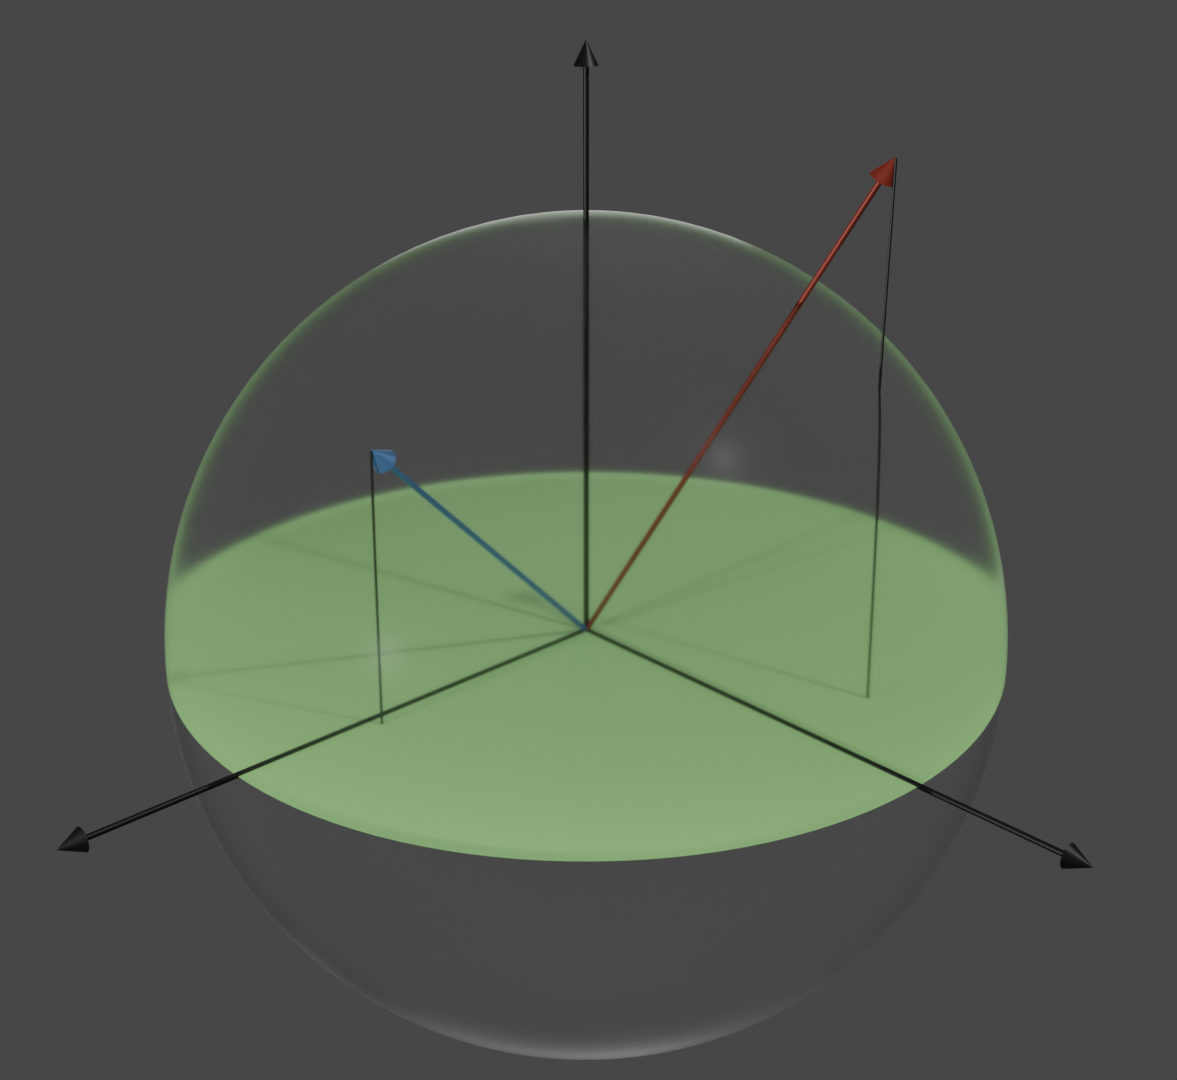
\includegraphics[width=0.75\textwidth]{figures/tiltSpherewBackground.png}
  \caption{\label{fig:tiltSphere} TODO}
\end{figure}

We now return to solving Eq. \eqref{eq:43}, using the solution angle we just found.
By insertion, and after some clean up, we get
\emph{note to thorvald: we chose \(\theta = Log \left(+ \dots\right) \)}
\begin{multline}
  \label{eq:52}
  (\exp[\Theta /2 \sigma_{x}] H_{B}\exp[\Theta /2 \sigma_{x}] - E \exp[\Theta \sigma_{x}]) \ket{\tilde{\psi}} = 0\\
  = v_F \begin{pmatrix}
          k_z ( s + t_z \gamma ) - E / v_F \gamma & -s ( ik_y + k_z t_x t_z \gamma - k_x / \gamma - E /v_{F} \gamma t_x)\\
          s ( i k_y - k_z t_x t_z \gamma + k_x / \gamma + E /v_F \gamma t_x) & - k_z (s - t_z \gamma) - E \gamma
        \end{pmatrix}\\
    \ket{\psi}.
\end{multline}
In order to simplify this further, absorb \(\gamma \beta (k_{z} t_{\parallel} - E /v_{F}) \) into \(k_{x}\).
Thus, let
\begin{equation}
  \label{eq:29}
  \begin{split}
    \tilde{k}_{x} &= k_{x} / \gamma + \gamma \beta ( E /v_F - k_{z} t_{\parallel}),\\
    \tilde{k}_{y} &=  k_{y},\\
    \tilde{k}_{z} &=  k_{z}.\\
  \end{split}
\end{equation}

These expressions warrant some explanation, as the Lorentz boost is of course
\begin{equation}
  \label{eq:23}
  \tilde{k_x} = \gamma (k_x - \beta \frac{E}{v_{F}}),
\end{equation}
where we used the four momentum \( p^{\mu } = (\frac{E}{v_{F}}, \vec{p}) \), and the effective speed of light \( v_F \).
It can thus look like our expression in Eq. \eqref{eq:29} is wrong.
The solution to this seeming inconsitency is that the proper energy is not \( \frac{E}{v_{F}} - k_z t_{\parallel} \), but rather \( \frac{E}{v_{F}} - k_z t_{\parallel} - k_x t_{\perp}\).
\todo{Something smart here}

The eigenvalue equation is simply
\begin{equation}
  \label{eq:53}
  \left[  \gamma \left( t_{\parallel} \tilde{k}_{z} - \frac{E}{v_{F}} \right) \mathcal{I}_{2} +
  s \tilde{k}_{i} \sigma _{i} \right] \ket{\tilde{\psi}}= 0.
\end{equation}
If we now again introduce the magnetic field using minimal coupling, \(k_{x} \to  k_{x} - ey B_{z} \), this corresponds to an effective field \(B_{z} \frac{v_{x} v_{y}}{v_{F}^2} / \gamma \) in the new quantities.
This is because \(\tilde{k}_{x} \to  \tilde{k}_{x} - e \tilde{y} \frac{v_{y} v_{x}}{v_{F}^2}  B_{z} /\gamma \), where the rescaled \(\tilde{y} = \frac{v_{F}}{v_{y}} y\).

The Landau level equation thus reads
\begin{equation}
  \label{eq:54}
  \left[
  \sum\limits_{i} s v_{F} \left(\tilde{k}_{i} + e \tilde{A}_{i} \right) \sigma _{i}
\right  ] \ket{\tilde{\psi}} =
(E- t_{\parallel} v_{F} \tilde{k}_{z}) \gamma \ket{\tilde{\psi}},
\end{equation}
where \(\vec{\tilde{A}}=-B_{z}/ \gamma  \tilde{y} \hat{x}\).
We may thus use directly the result for the untilted cone, \todo{eq ref}, giving
\begin{align}
  \label{eq:55}
  \left(E - t_{\parallel} v_{F} \tilde{k}_{z} \right) \gamma &= \sign (m) v_{F} \sqrt{2 |m| e \frac{B}{ \gamma } \hbar + \tilde{k}_{z}^2 \hbar ^2}, & m \neq 0,\\
  \left(E - t_{\parallel} v_{F} \tilde{k}_{z} \right) \gamma &= - s \hbar  \tilde{k}_{z} v_{F}, & m=0.
\end{align}
Cleaning up, we get
\begin{align}
  \label{eq:56}
  E &= t_{\parallel} v_F \tilde{k}_{z} + \sign(m) v_F \sqrt{2 |m| e \frac{B}{\gamma ^3} \hbar + \tilde{k}_{z}^2\hbar ^2 /\gamma ^2}, & m\neq 0,\\
  E &= \tilde{k}_{z} v_{F} \left( t_{\parallel}  - s \hbar / \gamma  \right), & m=0.
\end{align}

As the tilt is increased, \(\gamma = 1 / \sqrt{1-\beta ^{2}}\) diverges to infinity.
With the trivial substitution \(\alpha = \frac{1}{\gamma }\), which goes to zero, this gets an intuitive interpretation.
\begin{equation}
  \label{eq:57}
  E = t_{\parallel} v_{F} \tilde{k}_{z} + \sign(m) v_F \alpha \sqrt{2 |m| e B \alpha \hbar + \tilde{k}_{z}^2\hbar ^2}
\end{equation}
As the tilt increases, the Landau levels converge towards \(t_{\parallel} v_{F} \tilde{k}_{z}\).
\todo{Note that \( \tilde{k}\to 0 \) as we overtilt as well, so all the levels go to zero.}
In particular, the separation between Landau levels \(m\) \todo{maybe use the word cyclotron frequency} is reduced by a factor \(\alpha ^{\frac{3}{2}}\).
The effect of the tilt on the Landau levels is to squeeze the Landau levels together, and we will call the \(\alpha ^{\frac{3}{2}}\) the \emph{squeezing factor}.
We note that when approaching the degree of tilt where we are no longer able to find a boost which enables us to solve for the Landau levels, i.e. when \(\beta \to 1\), the squeezing factor goes to zero.
As the tilt exceeds this limit, the squeezing factor is imaginary.

Consider now isotropic velocities \( v_i = v_F \).
Even for anisotripic systems, we may rescale the momenta to arrive at such a description.
We may rewrite the energy as
\[
  E =
  \begin{cases}
    t_{\parallel} v_F k_z + \operatorname{sign}(m) v_F \alpha \sqrt{2 |m| e B \alpha + k_z^2} & m\neq 0\\
    t_{\parallel} v_F k_z - s \alpha v_F k_z & m=0,
  \end{cases}
\]
where \( \hbar = 1 \).
Notice that this is exactly
\[
E = t_{\parallel} v_F k_z + \alpha E^0_{m, \alpha B},
\]
where \( E^0_{m, B} \) is the energy in the untilted case, with magnetic field \( \alpha B \).

The eigenstate of
\[
H = v_{F} \sigma ^{i} ( p_{i} + e A_{i} ),
\]
with \(A_{i} = - B_{z} y \delta _{i x}\), given in the position basis, is
\begin{equation}
  \phi _{\vec{k} m s}(\vec{r}) = \frac{1}{\sqrt{L_xL_z}}
  \frac{e^{ik_x x}e^{ik_z z}}{\sqrt{\alpha _{k_z m s}^2 + 1}}
  e^{-\frac{y-k_x l^2}{2 l_B^2}}
  \begin{pmatrix}
    \frac{\alpha _{k_z m s}}{\sqrt{2^{M-1} (M-1)! \sqrt{\pi } l_B}} H_{M-1}\left( \frac{y-k_x l_B^2}{l_B} \right)\\
    \frac{1}{\sqrt{2^M M! \sqrt{\pi } l_B}} H_M \left( \frac{y-k_x l_B^2}{l_B} \right)
  \end{pmatrix},
\end{equation}
where capital letters indicate absolute value of corresponding quantity, $M=|m|, \vec{k} = (k_x, k_z)$, and with the normalization factor
\begin{equation}
  \alpha _{k_z m s} = \frac{-\sqrt{2eB\hbar M}}{\frac{E_{k_z m s}}{s v_{F}} - \hbar  k_z}.
\end{equation}
Taking care to keep track of boosted and rescaled quantites, the eigenstate in the boosted frame is
\begin{equation}
  \label{eq:58}
  \tilde{\psi}(\tilde{\vec{r}}) =
  \frac{1}{\sqrt{L_xL_z}}
  \frac{e^{i \tilde{k}_x \tilde{x}}e^{i k_z z}}{\sqrt{\alpha _{\tilde{k}_z m s}^2 + 1}}
  e^{-\frac{\left(\tilde{y} - \tilde{k}_x l_{B'}^2\right)^2}{2 l_{B'}^2}}
  \begin{pmatrix}
    \frac{\alpha _{\tilde{k}_z m s}}{\sqrt{2^{M-1} (M-1)! \sqrt{\pi } l_{B'}}} H_{M-1}\left( \frac{\tilde{y} - \tilde{k}_x l_{B'}^2}{l_{B'}} \right)\\
    \frac{1}{\sqrt{2^M M! \sqrt{\pi } l_{B'}}} H_M \left( \frac{\tilde{y} - \tilde{k}_x l_{B'}^2}{l_{B'}} \right)
  \end{pmatrix},
\end{equation}
with
\begin{equation}
  \alpha _{\tilde{k}_z m s} = \frac{-\sqrt{2e B' \hbar M}}{ \gamma \frac{E_{\tilde{k}_z m s} - t_{\parallel} v_{F} \tilde{k}_{z}}{s v_{F}} - \hbar  \tilde{k}_z},
\end{equation}
where
\[
B' = B \alpha.
\]
We note that \( \alpha_{k_z 0 s} = 0 \), so using the explicit form of the energy we may simplify the expression some.
For \( m\neq 0 \)
\[
  \frac{
    E_{k_z m s} - t_{\parallel} v_F k_z
  }{s v_{F}} = \sign(m) s \alpha \sqrt{2 M e B \alpha + k_{z}^2}
\]
and thus
\begin{equation}
  \label{eq:59}
  \alpha_{k_z m s} =
  \frac{-\sqrt{ \alpha M }}{\sign(m) s \sqrt{\alpha M + \kappa^2} - \kappa}
\end{equation}
where we defined the dimensionless \( \kappa_z = \sqrt{2 e B} k_z  \).


Note that


And thus the original eigenstate \(\ket{\psi } = 1 /\mathcal{N} e^{\theta /2 \sigma _{x}} \ket{\tilde{\psi} }\) of the tilted system is easily found.
The normalization factor \( \mathcal{N} \) is needed as the boost transformation is not unitary.

\todo{ Write down the full form of \( \phi _{\vec{k} m s} (\vec{r}) \), taking care to use the original momenta, and not the rescaled. }

Reinserting explicitly, in the boosted frame, that
\[
  \tilde{k}_{x} = \alpha k_{x} + \frac{\beta}{\alpha} (E_{k_z m s} /v_F- k_{z} t_{\parallel})
  = \alpha k_x + \beta \frac{E^0_{m, \alpha B} }{v_{F}}
\]
and \(l_{B'}=\frac{l_{B}}{\sqrt{\alpha} }\)
\begin{equation}
  \label{eq:60}
  \chi =
  \frac{y-\tilde{k}_{x} l_{B'}^2}{l_{B'}}
  =
  \sqrt{\alpha } (y-k_{x} l_{B}^2) /l_{B}
  - \frac{ \beta l_B }{ \sqrt{\alpha} v_F} E^{0}_{m, \alpha B}.
\end{equation}.
\todo{ Clean up in \(\hbar \) }


\begin{equation}
  \label{eq:61}
  \tilde{\phi} _{\vec{k} m s} (\vec{\tilde{r}})
  =
  \frac{1}{\sqrt{L_xL_z}}
  \frac{e^{i \tilde{k}_x \tilde{x}}e^{i k_z z}}{\sqrt{\alpha _{\tilde{k}_z m s}^2 + 1}}
  e^{-\frac{1}{2} \chi ^2}
  \sqrt[4]{\alpha }
  \begin{pmatrix}
    \frac{\alpha _{\tilde{k}_z m s}}{\sqrt{2^{M-1} (M-1)! \sqrt{\pi } l_{B}}} H_{M-1}\left( \chi  \right)\\
    \frac{1}{\sqrt{2^M M! \sqrt{\pi } l_{B}}} H_M \left( \chi \right)
  \end{pmatrix}.
\end{equation}
For later convenience, let us explicitly define
\begin{equation}
  \label{eq:62}
  \tilde{\phi} _{\vec{k} m s} (\vec{\tilde{r}}) =
  \frac{e^{i \tilde{k}_{x} \tilde{x} + i k_{z} z}}{\sqrt{L_{x} L_{z}} }
  \underbrace{
  \frac{
    e^{-\frac{1}{2} \chi ^2}
    \sqrt[4]{\alpha }
  }
  {\sqrt{\alpha^2_{\tilde{k}_{z} m s} + 1} }
  \begin{pmatrix}
    \frac{\alpha _{\tilde{k}_z m s}}{\sqrt{2^{M-1} (M-1)! \sqrt{\pi } l_{B}}} H_{M-1}\left( \chi  \right)\\
    \frac{1}{\sqrt{2^M M! \sqrt{\pi } l_{B}}} H_M \left( \chi \right)
  \end{pmatrix}}_{\tilde{\phi}_{\vec{k} m s} (y)},
\end{equation}
and thus
\begin{equation}
  \label{eq:63}
  \tilde{\phi}_{\vec{k} m s} (y) =
  e^{-\frac{1}{2} \chi ^2}
  \begin{pmatrix}
    a_{\vec{k} m s} H_{M-1} (\chi)\\
    b_{\vec{k} m s} H_{M} (\chi)
  \end{pmatrix},
\end{equation}
with
\begin{align}
 \label{eq:64}
  a_{\vec{k} m s} &=
                    \frac{
                    \alpha _{\tilde{k}_z m s} \sqrt[4]{\alpha }
                    }{
                    \sqrt{\alpha^2 _{\tilde{k}_z m s} + 1}
                    \sqrt{2^{M-1} (M-1)! \sqrt{\pi} l_B}
                    },\\
  b_{\vec{k} m s} &=
                    \frac{
                     \sqrt[4]{\alpha }
                    }{
                    \sqrt{\alpha^2 _{\tilde{k}_z m s} + 1}
                    \sqrt{2^{M} M! \sqrt{\pi} l_B}
                    }.\\
\end{align}

We proceed now to find the normalization factor \( \mathcal{N} \), as it will become necessary in later steps.
Recall that
\[
  \ket{\psi} = \frac{1}{\mathcal{N}} e^{\theta /2 \sigma _x} \ket{\tilde{\psi}},
\]
and
\[
e^{\theta \sigma _x} =
\frac{1}{\alpha }
\begin{pmatrix}
  1 & -s t_x\\
  -s t_x & 1
\end{pmatrix}.
\]
The upper and lower part of the spinor are orthogonal, thus we have
\begin{equation}
  \label{eq:65}
  \braket{\psi  | \psi } = \frac{1}{\mathcal{N}^{*} \mathcal{N}} \frac{1}{\alpha } \braket{\tilde{\psi}  | \tilde{\psi} } = 1 \implies \mathcal{N}^{*}\mathcal{N} = \frac{1}{\alpha }.
\end{equation}
We choose \( \mathcal{N} = \alpha^{-\frac{1}{2}} \).

\begin{Proposition}
  The tilted Hamiltonian
  \[
    H = v_F \vec{t} \vec{k} + s v_F \vec{k} \vec{\sigma}
  \]
  in a magnetic field \( \vec{B} \) has the Landau levels
  \[
    E =
    \begin{cases}
      t_{\parallel} v_F k_z + \sign(m) v_F \alpha \sqrt{2 e B \alpha M + k_{z} ^2} & m \neq 0\\
      t_{\parallel} v_F k_z - s \alpha v_F k_z & m = 0
    \end{cases}.
  \]
  The associated eigenstates in the position basis are
  \[
    \tilde{\psi}(\vec{r}) = \frac{1}{\mathcal{N}} e^{\theta /2 \sigma_x}
    \frac{
      e^{ik_{x} x + ik_{z} z}
    }{
      \sqrt{L_{x}  L_z}
    } \psi(y),
    \]
    where
    \[
      \psi(y) = e^{-\frac{1}{2} \chi^2}
      \begin{pmatrix}
        a_{k_z m s} H_{M - 1} (\chi) \\
        b_{k_z m s} H_M (\chi)
      \end{pmatrix},
    \]
    where we have defined \( \chi = \sqrt{\alpha} \frac{ y - k_x l_B^2 }{l_{B}} + \frac{\beta l_B}{\sqrt{\alpha} v_{F}} E^0_{m, \alpha B} \) and \( a_{k_z m s}, b_{k_z m s} \) are given in Eqs.~\eqref{eq:64}.
\end{Proposition}

\subsection{The energy momentum tensor}
The \emph{canonical} energy-momentum tensor is generally defined by
\begin{equation}
  \label{eq:19}
  T^{\mu \nu} =  \frac{\delta \mathcal{L}}{\delta(\partial_{\mu} \phi_{i})} \partial_{\nu} \phi_i - \eta^{\mu \nu} \mathcal{L},
\end{equation}
where the index \( i \) runs over the types of fields.
This definition is correct for commuting fields, however, for non-commuting fields like ours, this formula is slightly wrong.
This is often overlooked in many textbooks and papers, so we will here elucidate the issue to some degree.
While a proper derivation requires the use of Grassman variables and defining left and right derivation, which we will not do here, some simple considerations help in understanding the issue.
In the standard text book derivation of then canonical energy-momentum tensor, one expands the total derivative of the Lagrangian \( \mathcal{L}(\psi_i, \partial \psi_i)\) in terms of the fields
\begin{equation}
  \label{eq:30}
  \frac{\mathrm{d} \mathcal{L}(\psi_{i}, \partial \psi_i)}{\mathrm{d} x_{\nu }} \equiv \mathrm{d}^{\nu } \mathcal{L}
  = \frac{\partial \mathcal{L}}{\partial (\partial_{\mu } \phi_i)} \frac{\partial(\partial _{\mu } \psi_i)}{\partial x_{\nu }}
  + \frac{\partial \mathcal{L}}{\partial \psi _{i}} \frac{\partial \psi_i}{\partial x_{\nu }}.
\end{equation}
This expansion, however, ignores the non-commutative nature of the fields.
For concreteness, consider \( \psi _i = \bar{\psi} \).
Heuristically, the correct expression would be obtained by reordering the factors in the two terms.
By naively employing Eq. \eqref{eq:19}, the resulting canonical energy-momentum tensor of the Dirac theory would be
\begin{equation}
  T^{\mu \nu} = \frac{\delta \mathcal{L}}{\delta (\partial_{\mu} \bar{\psi})} \partial^{\nu} \bar{\psi}  + \frac{\delta \mathcal{L}}{\delta (\partial_{\mu} \psi)} \partial^{\nu} \psi - \eta^{\mu \nu} \mathcal{L},
\end{equation}
while the correct form is \cite[Eq.~3-153]{itzyksonQuantumFieldTheory1980}
\begin{equation}
  \label{eq:21}
  T^{\mu \nu} = \partial^{\nu} \bar{\psi} \frac{\delta \mathcal{L}}{\delta (\partial_{\mu} \bar{\psi})} + \frac{\delta \mathcal{L}}{\delta (\partial_{\mu} \psi)} \partial^{\nu} \psi - \eta^{\mu \nu} \mathcal{L}.
\end{equation}

Our Hamiltonian
\[
H_s = s \sigma^i k_i
\]
may of course be considered as a Weyl decomposition of a full massless Dirac equation.

\todo{Why do we have to consider 4x4? Is the definitions not also valid for 2x2?}
\todo{Regarding the non-symmetry of the stress tensor, see keichelriess eq 5.16 with discussion}

The Hamiltonian
\[
H_s = s \sigma^i k_i
\]
can be considered the Hamiltonian of one part of a Weyl decomposition of a Dirac system.
The Weyl field has the Lagrangian density \cite{kachelriessQuantumFieldsHubble2018}
\begin{equation}
  \label{eq:18}
  \mathcal{L} = i \phi^{\dagger} \sigma^{\mu} \partial_{\mu} \phi,
\end{equation}
which may be seen directly from the Dirac Lagrangian \( i \bar{\psi} \slashed{\partial } \psi  \) by taking \( \psi = (\phi_L, \phi_R)^T \) and set, for example, \( \phi _R = 0 \).
Symmetrizing in daggered and undaggered fields
\footnote{The Lagrangian itself is unphysical, and we may transform it in any way that leaves the action \( \int \mathcal{L} \) invariant.}
\todo{Alternatively argue by directly showning that this does not affect the action by doing an integration by parts}
\[
  \mathcal{L} = \frac{i}{2} \left(\phi^{\dagger} \sigma^{\mu} \partial_{\mu} \phi - \partial_{\mu} \phi^{\dagger} \sigma^{\mu} \phi \right),
\]
which will prove to be more convenient to work with.
Adapting the definition Eq. \eqref{eq:21} the energy-momentum tensor for the untilted Dirac cone is thus
\begin{equation}
  \label{eq:20}
  T^{\mu \nu} =
  \frac{i}{2} (
  \phi^{\dagger} \sigma^{\mu} \partial_{\nu} \phi
  - \sigma^{\mu} \phi \partial_{\nu} \phi^{\dagger}
  - \eta^{\mu \nu} \mathcal{L}
  ).
\end{equation}

Moving now to the tilted case, the 4x4 Lagrangian becomes \cite{vanderwurffMagnetovorticalThermoelectricTransport2019}
\todo{check sign compared to action in stoof}
\begin{equation}
  \label{eq:31}
  \mathcal{L}_{\text{tilt}} = i \bar{\psi} \Gamma ^{\mu }\partial_{\mu } \psi ,
\end{equation}
where we have introduced modified gamma matrices
\begin{equation}
  \label{eq:107}
  \Gamma ^{\mu } =
  \begin{cases}
    \gamma ^{\mu } + t^{\mu} \gamma ^0& \text{ inversion symmetry broken },\\
    \gamma^{\mu} + t^{\mu} \gamma^0 \gamma^5 & \text{ inversion symmetric },
  \end{cases}
\end{equation}
with \( t^{\mu } = (0, \vec{t}) \).
\begin{equation}
  \label{eq:108}
  T^{\mu \nu} =
  \frac{i}{2} (
  \phi^{\dagger} \tilde{\sigma} ^{\mu} \partial_{\nu} \phi
  - \tilde{\sigma} ^{\mu} \phi \partial_{\nu} \phi^{\dagger}
  - \eta^{\mu \nu} \mathcal{L}
  ),
\end{equation}
where we defined the modified Pauli matrices
\begin{equation}
  \label{eq:109}
  \tilde{\sigma}^{\mu} =
  \begin{cases}
    \sigma^{\mu} + t^{\mu} & \text{ inversion symmetry broken },\\
    \sigma^{\mu} + s t^{\mu} & \text{ inversion symmetric }.
  \end{cases}
\end{equation}



\section{The response of a tilted cone}

Repeating the calculation of the response function is now straightforward, but rather tedious.
Due to the boost transformation, the elements of the spinor in the untilted system, Eq. \eqref{eq:58}, mix.
We thus have twice as many terms to keep track of.

Consider the expression for the current operator, Eq. 4.39, which we derived form the time evolution relation
\[
  \dot{A} = [A, H]/i\hbar,
\]
by considering \(\vec{v} = \vec\dot{r}\), as \(\vec{J} = e \vec{v}\).
In the tilted Hamiltonian, the tilt term thus causes another term in the current operator.
\begin{equation}
  \label{eq:66}
  \begin{split}
    \vec{v} = \vec\dot{r} &= \frac{1}{i \hbar } [\vec{r}, H] \\
    &= \frac{s v_{F} \sigma ^{ i}}{i \hbar } [\vec{r}, p_{i} + e A_{i}] + \frac{1}{i\hbar } [\vec{r}, \omega_{0} \vec{k}]\\
    &= \frac{s v_{F} \sigma ^{ i}}{i \hbar } (i\hbar + e[\vec{r}, A_{i}]) + \vec{\omega}_{0}\\
    &= s v_{F} \sigma ^{i} + \vec{\omega} _{0}.
  \end{split}
\end{equation}

Take for example the matrix element of the current operator
\[
  J_{\vec{k} m s; \vec{k}+\qvec{q} n s } (\vec{q}) = \int \mathrm{d}y e^{-i q_{y} y}
  s v_{F} e \phi ^{*}_{\vec{k} m s} (y) \sigma ^{x} \phi _{\vec{k} + \qvec{q} n s}(y).
\]
We must find the matrix product \(\phi \sigma_{x} \phi \).
Recall that \(\phi = \frac{1}{\mathcal{N}} e^{\theta /2 \sigma _{x}} \tilde{\phi} \), and thus we must find
\[
  \phi ^{*} \sigma _{x} \phi = \frac{1}{\mathcal{N}^{*} \mathcal{N}} \tilde{\phi}^{*} e^{\theta /2 \sigma _{x}} \sigma _{x} e^{\theta /2 \sigma _{x}} \tilde{\phi} =  \frac{1}{\mathcal{N}^{*} \mathcal{N}} \tilde{\phi}^{*} \sigma _{x} e^{\theta \sigma _{x}} \tilde{\phi}.
\]
With the previously found solution \(\theta = - \tanh ^{-1} t_{x}\), we get the rather simple form
\[
  e^{\theta \sigma _{x}} =
  \begin{pmatrix}
    1 & - s t_{x}\\
    -s t_{x} & 1
  \end{pmatrix}
  \frac{1}{\sqrt{1-t_{x}^2}}.
\]
With
\begin{equation}\label{eq:67}
  \tilde{\phi} = e^{-\frac{1}{2} \chi ^2}
  \begin{pmatrix}
    a_{\vec{k} m s} H_{M-1} (\chi)\\
    b_{\vec{k} m s} H_{M} (\chi)
  \end{pmatrix}
\end{equation}
we see how the expressions change when \(t_{x}\) become non-zero.
Where we previoulsy had
\begin{equation}
  \label{eq:68}
  \phi ^{*}_{\vec{k} m s} \sigma _{x} \phi _{\vec{k} + \qvec{q} n s}
  =
  a_{\vec{k} m s} H_{M-1}(\dots) \left[ b_{\vec{k}+\qvec{q} n s} H_{N}(\dots) \right]
  + \dots
\end{equation}
the contents of the square brackets must now include also the other element of the spinor:
\begin{equation}
  \label{eq:69}
  \phi ^{*}_{\vec{k} m s} \sigma _{x} e^{\theta \sigma _{x}} \phi _{\vec{k} + \qvec{q} n s}
  =
  a_{\vec{k} m s} H_{M-1}(\dots)
  \left[
    b_{\vec{k}+\qvec{q} n s} H_{N}(\dots)
    - s t_{x} a_{\vec{k} + \qvec{q} n s} H_{N-1} (\dots)
  \right]
  \frac{1}{\sqrt{1-t_{x}^2}}
  + \dots .
\end{equation}

First of all, let us consider the exponent of the product.
Due to the extra term in \(\chi\), this becomes more elaborate.
The exponent is of course
\begin{equation}
  \label{eq:70}
  \exp\{-i q_{y} y - \frac{1}{2} \chi_{\vec{k}} ^2 - \frac{1}{2} \chi _{\vec{k} + \qvec{q}}^2\}
\end{equation}
A straightforward but tedious calculation shows that the argument of the exponent can be written as
\begin{equation}
  \label{eq:71}
  -\frac{\alpha}{l_{B}^2} \left(y + \frac{l_{B}^2}{2 \alpha } (i q_{y} - (q'_x + 2 k'_x))\right)^2
  -\frac{l_{B}^2}{4 \alpha } (q_{y}^2 + 2i (q'_x + 2 k'_x) q_{y} + ( q' _{x} )^2 ),
\end{equation}
where we have defined
\begin{align}
  \label{eq:qkprime}
  q' _x &= q_x \alpha  - \frac{\beta}{v_{F} }( E^0_{n,\alpha B} - E^0_{m, \alpha B} ),\\
  k' _x &= k_x\alpha - \frac{\beta}{v_F } E^0_{m, \alpha B}.
\end{align}
These must not be confused with the transformed momenta \( \tilde{k} \), which are similar in form.
Eq. \eqref{eq:71} is on the same for as in the untilted cone case, and we may thus proceed with the same method.
Make a change of variable
\[
\tilde{y} = \frac{\sqrt{\alpha }}{l_{B}} \left(y + \frac{l_{B}^2}{2\alpha } (iq_{y} - 2 k' _x - q' _x )\right),
\]
\todo{Follow up the substitution of the root in the integral. Consider moving the root into \(\Xi \)}
to get the exponent on the form \(e^{-\tilde{y}^2}\).
With this substitution,
\begin{align}
  \chi _{\vec{k}} &= \tilde{y} + \frac{l_{B}}{2 \sqrt{\alpha }} \left(q' _x - i q_{y}\right)\\
  \chi _{\vec{k} + \qvec{q}} &= \tilde{y} + \frac{l_{B}}{2 \sqrt{\alpha }} \left(- q' _x - i q_{y}\right)
\end{align}

Doing this, Eq. (4.59) \todo{fix ref} in the project thesis, becomes
\begin{equation}
  \begin{split}
    J_{\vec{k}ms; \vec{k}+\qvec{q} ns}(\vec{q}) &=
    \frac{s v_F e}{\sqrt{\alpha }} \int \mathrm{d}\tilde{y} \: l_B
    \exp \left[
      -\frac{l_{B}^2}{4 \alpha } \left(q_{y}^2 + 2i (2 k' _x + q' _x) q_{y} + (q'_x)^2 \right)
    \right]
   \\
    e^{-\tilde{y}^2}
   &\left[
    a_{\vec{k}ms}b_{\vec{k} + \qvec{q} ns}
    H_{M-1} \left(  \chi_{\vec{k}} \right)
    H_N\left( \chi_{\vec{k} + \qvec{q}} \right) \right.\\
    &- s t_{x} a_{\vec{k}ms}a_{\vec{k} + \qvec{q} ns}
    H_{M-1} \left( \chi_{\vec{k}} \right)
    H_{N-1}\left( \chi_{\vec{k} + \qvec{q}} \right)\\
   & +
    b_{\vec{k}ms} a_{\vec{k} + \qvec{q} ns}
    H_M \left( \chi_{\vec{k}} \right)
    H_{N-1} \left( \chi_{\vec{k} + \qvec{q}} \right)\\
    &\left. - s t_{x}
    b_{\vec{k}ms} b_{\vec{k} + \qvec{q} ns}
    H_M \left( \chi_{\vec{k}} \right)
    H_{N} \left(  \chi_{\vec{k} + \qvec{q}}\right)
    \right],
  \end{split}
\end{equation}
where we used \( \mathcal{N}^{*}\mathcal{N} \alpha = 1 \)

\begin{multline}
  J_{\vec{k} m s; \vec{k} + \qvec{q} n s} (\vec{q}) =
  s v_{F} e
  \frac{
    \exp \left[
      -\frac{l_{B}^2}{4 \alpha } (q_{y}^2 + 2i (2 k'_x + q'_x) q_{y} + (q'_x)^2 )
    \right]
  }{
    \sqrt{\alpha _{\vec{k} m s}^2 + 1} \sqrt{ \alpha _{\vec{k} + \qvec{q} n s}^2 + 1 }
  } \\
  % \sum\limits_{i=1}^{4} \chi_{i} (\vec{q}, m, n, s)
  \Big[
   \alpha _{\vec{k} m s} \Xi_{1} (\vec{q}, m, n, s)
    + \alpha _{\vec{k} + \qvec{q} n s} \Xi _{2} (\vec{q}, m, n, s)\\
    -s t_x \alpha _{\vec{k} m s} \alpha _{\vec{k} + \qvec{q} n s} \Xi _1(\vec{q}, m, n\mp 1, s)
    -s t_x \Xi _2(\vec{q}, m, n\pm 1, s)
  \Big].
\end{multline}

We here used definitions of \( \Xi \) similar to that in the project thesis, but modified to the tilted case.
\begin{equation}
  \label{eq:72}
  \frac{ \sqrt{\alpha } \alpha _{\vec{k} m s} \Xi_1 ( \vec{q}, m, n, s )}{
    \sqrt{\alpha _{\vec{k} m s}^2 + 1}
    \sqrt{\alpha _{\vec{k} + \qvec{q} n s} ^2 + 1}
  }
  =
  \int \mathrm{d} \tilde{y}
  ~e^{-\tilde{y}^2}
  l_{B}
  a_{\vec{k} m s} b_{\vec{k} + \qvec{q} ns}
  H_{M-1} (\chi_{\vec{k}})
  H_N ( \chi _{\vec{k} + \qvec{q}} )
\end{equation}
\begin{equation}
  \label{eq:73}
  \frac{ \sqrt{\alpha } \alpha _{\vec{k} + \vec{q} n s} \Xi_2 ( \vec{q}, m, n, s )}{
    \sqrt{\alpha _{\vec{k} m s}^2 + 1}
    \sqrt{\alpha _{\vec{k} + \qvec{q} n s} ^2 + 1}
  }
  =
  \int \mathrm{d} \tilde{y}
  ~e^{-\tilde{y}^2}
  l_{B}
  b_{\vec{k} m s} a_{\vec{k} + \qvec{q} ns}
  H_{M} (\chi_{\vec{k}})
  H_{N-1} ( \chi _{\vec{k} + \qvec{q}} )
\end{equation}

Recall the \emph{shifted orthogonality} relation for Hermite polynomials~\cite[Eq. (7.377)]{gradshteinTableIntegralsSeries2015}
\begin{equation}
  \label{eq:hermite-shift-ortho}
  \int\limits_{-\infty }^{\infty } \mathrm{d}x
  e^{-x^2} H_m(x+y) H_n(x+z)
  = 2^n \pi^{\frac{1}{2}} m! y^{n-m} L^{n-m}_m(-2yz), \quad m\leq n,
\end{equation}
where \(L^{a}_{b}\) is the \emph{generalized Laguerre polynomial} of order \(b\) and type \(a\).
Using that
\begin{align}
  a_{\vec{k} m s} b_{\vec{k} +\qvec{q} ns}
  &=
    \sqrt{\alpha } \frac{\alpha_{\vec{k} m s}}{\sqrt{\alpha _{\vec{k} m s} ^2 + 1} \sqrt{\alpha _{\vec{k} + \qvec{q} ns} ^2  + 1}  }
    \left[
    2^{N+M-1} (M-1)! N! \pi l_{B}^2
    \right  ]^{-\frac{1}{2}}\\
  b_{\vec{k} m s} a_{\vec{k} +\qvec{q} ns}
  &=
    \sqrt{\alpha } \frac{\alpha_{\vec{k} + \qvec{q} n s}}{\sqrt{\alpha _{\vec{k} m s} ^2 + 1} \sqrt{\alpha _{\vec{k} + \qvec{q} ns} ^2  + 1}  }
    \left[
    2^{N+M-1} (N-1)! M! \pi l_{B}^2
    \right  ]^{-\frac{1}{2}}\\
  a_{\vec{k} m s} a_{\vec{k} +\qvec{q} ns}
  &=
    \sqrt{\alpha } \frac{\alpha_{\vec{k} m s} \alpha_{\vec{k} + \qvec{q} n s}}{
    \sqrt{\alpha _{\vec{k} m s} ^2 + 1} \sqrt{\alpha _{\vec{k} + \qvec{q} ns} ^2  + 1}
    }
    \left[
    2^{N+M-2} (M-1)! (N-1)! \pi l_{B}^2
    \right  ]^{-\frac{1}{2}}\\
  b_{\vec{k} m s} b_{\vec{k} +\qvec{q} ns}
  &=
    \sqrt{\alpha } \frac{1}{
    \sqrt{\alpha _{\vec{k} m s} ^2 + 1} \sqrt{\alpha _{\vec{k} + \qvec{q} ns} ^2  + 1}
    }
    \left[
    2^{N+M} M! N! \pi l_{B}^2
    \right  ]^{-\frac{1}{2}}\\
\end{align}
\todo{NB!! definition changed compared to project thesis. Here, we have dropped the \( \alpha  \) factor}
\todo{Verify if we need to add some factors due to the tilt.}
\begin{align}
  \Xi_1 ^{(1)}(\vec{q}, m, n, s) &= \sqrt{\frac{2^N (M-1)!}{2^{M-1} N!}}
                                   \left( \frac{q'_x - iq_y}{2 \sqrt{\alpha } } l_B \right)^{N-M + 1}
                                   L^{N-M+1}_{M-1} \left( \frac{\qvec{q}_y^2 l_B^2}{2 \alpha } \right),\\
                                   %%%
  \Xi_1 ^{(2)}(\vec{q}, m, n, s) &= \sqrt{\frac{2^{M-1} N!}{2^N (M-1)!}}
                                   \left( \frac{-q'_x - iq_y}{2 \sqrt{\alpha } } l_B \right)^{M-N - 1}
                                   L^{M - N - 1}_N \left( \frac{\qvec{q}_y^2 l_B^2}{2 \alpha } \right),\\
  \Xi_1(\vec{q}, m, n, s) &=
          \begin{cases}
            \Xi _1 ^{(1)} & \text{if } N \geq M-1\\
            \Xi _1 ^{(2)} & \text{if } N \leq M-1
          \end{cases},
\end{align}
\begin{align}
  \Xi_2 ^{(1)}(\vec{q}, m, n, s) &= \sqrt{\frac{2^{N-1} M!}{2^M (N-1)!}}
                                   \left( \frac{q'_x - iq_y}{2 \sqrt{\alpha }} l_B \right)^{N-1 - M}
                                   L^{N-1 -M}_{M} \left( \frac{\qvec{q}_y^2 l_B^2}{2 \alpha } \right),\\
                                   %%%
  \Xi_2 ^{(2)}(\vec{q}, m, n, s) &= \sqrt{\frac{2^M (N-1)!}{2^{N-1} M!}}
                                   \left( \frac{-q'_x - iq_y}{2 \sqrt{\alpha }} l_B \right)^{M-N + 1}
                                   L^{M - N + 1}_{N-1} \left( \frac{\qvec{q}_y^2 l_B^2}{2 \alpha } \right),\\
  \Xi_2(\vec{q}, m, n, s) &=
          \begin{cases}
            \Xi _2 ^{(1)} & \text{if } N-1 \geq M\\
            \Xi _2 ^{(2)} & \text{if } N-1 \leq M
          \end{cases},
\end{align}
Here, \( \qvec{q}_y = (q'_x, q_y) \).
\todo{In the future, might be nice to go over to having only one function, Xi1, and simply mix around the arguments}


Now we will consider the second term of the current operator.
\begin{equation}
  \label{eq:74}
  J_{\vec{k} m s; \vec{k} + \qvec{q} n s}^{(2)} (\vec{q}) =
  \int \mathrm{d} y
  e^{-iq_{y} y} e
  \phi ^{*}_{\vec{k} m s}(y) \omega _{0 x} \phi _{\vec{k} + \qvec{q} n s}(y).
\end{equation}
Thus
\begin{multline}
  \label{eq:75}
  J_{\vec{k} m s; \vec{k} + \qvec{q} n s}^{(2)} (\vec{q}) =
  \frac{e v_F t_x }{\mathcal{N}^{*} \mathcal{N}}
  \int \mathrm{d} y
  \exp\{-i q_{y} y - \frac{1}{2} \chi_{\vec{k}} ^2 - \frac{1}{2} \chi _{\vec{k} + \qvec{q}}^2\} \\
  \tilde{\phi} ^{*}_{\vec{k} m s}(y) e^{\theta \sigma _{x}} \tilde{\phi} _{\vec{k} + \qvec{q} n s}(y).
\end{multline}
Using the same substitution and completion of the square as above, this is
\begin{multline}
  \label{eq:76}
  J_{\vec{k} m s; \vec{k} + \qvec{q} n s}^{(2)} (\vec{q}) =
  \frac{e v_F t_x l_{B}}{\sqrt{\alpha}}
  \int \mathrm{d} \tilde{y}
    \exp \left[
      -\frac{l_{B}^2}{4 \alpha } (q_{y}^2 + 2i (2 k'_x + q' _x) q_{y}  + (q'_x)^2 )
    \right]\\
  e^{-\tilde{y}^2} \big[
    a_{\vec{k} m s} H_{M-1}( \chi _{\vec{k}} ) \left(a_{\vec{k} + \qvec{q} n s} H_{N-1}( \chi _{\vec{k} + \qvec{q}} ) - s t_{x} b_{\vec{k} + \qvec{q} n s} H_{N}( \chi _{\vec{k} + \qvec{q}} ) \right)\\
   +
    b_{\vec{k} m s} H_{M}( \chi _{\vec{k}} ) \left(- s t_{x} a_{\vec{k} + \qvec{q} n s} H_{N-1}( \chi _{\vec{k} + \qvec{q}} ) + b_{\vec{k} + \qvec{q} n s} H_{N}( \chi _{\vec{k} + \qvec{q}} ) \right)
    \big].
\end{multline}
Thus
\footnote{Note to self: note that we dropped the \( \frac{1}{\sqrt{\alpha } } \) for the \( \sqrt{\alpha }  \) coming from the \( \Xi  \) definition.}
\begin{multline}
  J_{\vec{k} m s; \vec{k} + \qvec{q} n s}^{(2)} (\vec{q}) =
  e v_F t_x
  \frac{
    \exp \left[
      -\frac{l_{B}^2}{4 \alpha } (q_{y}^2 + 2i (2 k' _x + q' _x) q_{y} + (q'_x)^2 )
    \right]
  }{
    \sqrt{\alpha_{\vec{k} m s}^2 + 1} \sqrt{\alpha _{\vec{k}+\qvec{q} n s}^2 + 1}
  }\\
  \Big[
  -s t_x [ \alpha_{\vec{k} m s} \Xi_1(\vec{q}, m, n) + \alpha_{\vec{k} + \qvec{q} n s} \Xi_2(\vec{q}, m, n) ]\\
  + \alpha_{\vec{k} m s} \alpha_{\vec{k} + \qvec{q} ns} \Xi_1(\vec{q}, m, n\mp 1)
  + \Xi_2(\vec{q}, m, n \pm 1) \Big].
\end{multline}
We notice that this part has the same form as \( J^{(1)} \), with only a change of the prefactors of the \( \Xi  \)-functions.
\emph{Note to self: } I believe it is here important to consider if we have an inversion symmetric or inversion unsymmetric case. In the former, this makes everything easier, as the nasty terms are dropped.

\begin{multline}
  J_{\vec{k} m s; \vec{k} + \qvec{q} n s} (\vec{q}) =
  e v_F s \alpha^2
  \frac{
    \exp \left[
      -\frac{l_{B}^2}{4 \alpha } (q_{y}^2 + 2i (2 k' _x + q' _x) q_{y} + (q'_x)^2 )
    \right]
  }{
    \sqrt{\alpha_{\vec{k} m s}^2 + 1} \sqrt{\alpha _{\vec{k}+\qvec{q} n s}^2 + 1}
  }\\
  \left[
     \alpha_{\vec{k} m s} \Xi_1(\vec{q}, m, n) + \alpha_{\vec{k} + \qvec{q} n s} \Xi_2(\vec{q}, m, n)
  \right].
\end{multline}
We used here that \( 1 - t_x^2 = \alpha^2 \).

\subsubsection{Stress-energy tensor}
Consider now
\begin{equation}
  \label{eq:77}
  T_{\vec{k} + \qvec{q} n s, \vec{k} m s}^{0y(1)} (\vec{q}) =
  \frac{1}{4}
  \int \mathrm{d} y
  e^{i q_{y} y}
  \phi ^{*}_{\vec{k} + \qvec{q} n s}(y) s \sigma ^{y}
  (E_{k \mu  s} + E_{\lambda \nu s} - 2 \mu)
  \phi _{\vec{k} m s} (y).
\end{equation}
As
\begin{equation}
  \label{eq:78}
  % e^{\theta /2 \sigma _{x}} \sigma _{y} e^{\theta /2 \sigma _{x}} = 1
  \sigma _{y} e^{\theta /2 \sigma _{x}} = e^{-\theta /2 \sigma _{x}} \sigma _{y}
\end{equation}
we get the very fortunate result
\begin{equation}
  \label{eq:79}
  \phi^{*} \sigma _{y} \phi = \frac{1}{\mathcal{N}^{*} \mathcal{N}} \tilde{\phi}^{*} \sigma _{y} \tilde{\phi}.
\end{equation}
The first term of the stress-energy tensor thus has the exact same form as the untilted case.
Recalling the expression for \(\tilde{\phi}\) from Eq. \eqref{eq:67},
\[
  \tilde{\phi} = e^{-\frac{1}{2} \chi ^2}
  \begin{pmatrix}
    a_{\vec{k} m s} H_{M-1} (\chi)\\
    b_{\vec{k} m s} H_{M} (\chi)
  \end{pmatrix},
\]
where
\[
\chi = \sqrt{\alpha} (y - q_{x} l_{B}^2 ) /l_{B} - \sign(m) \beta \sqrt{2 |m| + \frac{k_{z}^2 l_{B}^2}{\alpha }}.
\]
We thus get
\begin{multline}
  \label{eq:80}
  T_{\vec{k}+\qvec{q} ns, \vec{k} m s}^{0y (1)} (\vec{q}) =
  \frac{is}{4 \mathcal{N}^{*}\mathcal{N}} (E_{k\mu  s} + E_{\lambda \nu s} - 2 \mu)
  \int \mathrm{d} y
  e^{i q_{y} y}
  e^{-\frac{1}{2} (\chi_{\vec{k}+\qvec{q}}^2 + \chi_{\vec{k}} ^2) }\\
  [
  -a_{\vec{k} + \qvec{q} ns} b_{\vec{k} m s} H_{N-1} (\chi_{\vec{k} + \qvec{q}}) H_{M} (\chi_{\vec{k}})
  + b_{\vec{k} + \qvec{q} n s} a_{\vec{k} ms} H_{N}(\chi_{\vec{k} + \qvec{q}}) H_{M-1} (\chi_{\vec{k}})
  ].
\end{multline}
We will perform once again the completion of the square and substituion of \(y\).
The exponent is the same as that which we found for the current operator case, Eq. \eqref{eq:71}, with the change \(q_{y} \to - q_{y}\).
We thus make the change of variables
\begin{equation}
  \label{eq:81}
  \tilde{y} = \frac{\sqrt{\alpha}}{l_{B}} \left(y  - \frac{l_{B}^2}{2 \alpha } (i q_{y} + (2k' _x + q' _x) )\right),
\end{equation}
giving
\begin{align}
  \chi _{\vec{k}} &= \tilde{y} + \frac{l_{B}}{2 \sqrt{\alpha }} \left( q'_x + i q_{y}\right),\\
  \chi _{\vec{k} + \qvec{q}} &= \tilde{y} + \frac{l_{B}}{2 \sqrt{\alpha }} \left( -q' _{x} + i q_{y}\right).
\end{align}
Thus, analogous to Eq. (4.79), we get
\begin{multline}
  \label{eq:82}
  T_{\vec{k} + \qvec{q} n s, \vec{k} m s}^{0y (1)} (\vec{q}) =\\
  \frac{is}{4 \mathcal{N}^{*}\mathcal{N} \sqrt{\alpha} }
  (E_{k\mu s} + E_{\lambda  \nu  s} - 2 \mu)
  \exp \left[
    -\frac{l_{B}^2}{4 \alpha } (q_{y}^2 - 2i (2 k' _x + q' _x) q_{y} + (q' _x)^2 )
  \right  ]
  \int \mathrm{d} \tilde{y} l_{B} e^{-\tilde{y}^2}\\
 \Big[
  - a_{\vec{k} + \qvec{q} ns} b_{\vec{k} m s}
  H_{N-1} ( \chi _{\vec{k}} )
  H_{M} ( \chi _{\vec{k} + \qvec{q}} )
  + b_{\vec{k} + \qvec{q} ns } a_{\vec{k} m s}
  H_{N}( \chi _{\vec{k}} )
  H_{M-1} ( \chi _{\vec{k} + \qvec{q}} )
  \Big]
\end{multline}
And thus we have
\begin{align}
  T_{\vec{k} + \qvec{q} n s, \vec{k} m s}^{0y (1)} (\vec{q}) &=
  \frac{is \alpha }{4  }
  \frac{E_{k\mu s} + E_{\lambda  \nu  s} - 2 \mu}{
    \sqrt{\alpha _{\vec{k} m s}^2 + 1}
    \sqrt{\alpha _{\vec{k} + \qvec{q} n s}^2 + 1}
  }\\
  &\pe \exp \left[
    -\frac{l_{B}^2}{4 \alpha } (q_{y}^2 - 2i ( 2k' _x + q' _x ) q_{y} + (q' _x)^2)
  \right  ]\\
  &\pe (-\alpha_{\vec{k}+\qvec{q} n s} \Xi_{2} (\bar{\vec{q}}, m, n, s) + \alpha_{\vec{k} m s} \Xi_{1}(\bar{\vec{q}}, m, n, s)),
\end{align}
where \(\bar{\vec{q}} = (q_{x}, -q_{y}, q_{z})\).

We must now consider the latter parts of the stress energy tensor
\begin{align}
  T_{\vec{k} + \qvec{q} ns, \vec{k} ms}^{0y (2)} (\vec{q}) &=
                                                             + \frac{1}{4} \int \mathrm{d} y
                                                             e^{iq_{y} y} v_{F}
                                                             \phi ^{*}_{\vec{k}+\qvec{q} ns} (y) p_{y} \phi _{\vec{k} m s} (y),\\
  T_{\vec{k} + \qvec{q} ns, \vec{k} ms}^{0y (3)} (\vec{q}) &=
                                                             - \frac{1}{4} \int \mathrm{d} y
                                                             e^{iq_{y} y} v_{F}
                                                             (p_{y} \phi ^{*}_{\vec{k}+\qvec{q} ns} (y))  \phi _{\vec{k} m s} (y).
\end{align}
Firstly, we note that
\[
  [p_{y} , e^{\theta /2 \sigma _{x}}] = 0.
\]
Furthermore, exactly as for the untilted case, the momentum operator acting on the exponential prefactor of \(\phi \) gives contributions proportional to \(q_{x}\).
In the local limit \(q\to  0\) this term vanishes, and we need only consider the effect of the momentum operator acting on the Hermite polynomials.

Denote by \(\tilde{p}_{y}\) the momentum operator \(p_{y}\) acting only on the Hermite polynomial part of \(\phi \).
Furthermore, we will use the property of Hermite polynomials \(\partial _{x} H_{n} (x) = 2 n H_{n-1} (x)\) \cite[Eq.~18.9.25]{NIST:DLMF}.
\begin{align}
  \tilde{p}_{y} \phi _{\vec{k} ms} &=
  -i \hbar
  e^{\theta /2 \sigma _{x}}
  e^{-\frac{1}{2} \chi ^2}
  \partial _{y}
  \begin{pmatrix}
    a_{\vec{k} m s} H_{M-1} (\chi) \\
    b_{\vec{k} ms} H_{M} (\chi)
  \end{pmatrix}\\
                                   &=
                                     -i \hbar
                                     e^{\theta /2 \sigma _{x}}
                                     e^{-\frac{1}{2} \chi ^2}
                                     2 \frac{\partial \chi }{\partial y}
                                     \begin{pmatrix}
                                       a_{\vec{k} m s} (M-1) H_{M-2} (\chi) \\
                                       b_{\vec{k} ms} (M) H_{M-1} (\chi)
                                     \end{pmatrix}\\
                                   &=
                                     -i \hbar
                                     e^{\theta /2 \sigma _{x}}
                                     e^{-\frac{1}{2} \chi ^2}
                                     \frac{2 \sqrt{\alpha}}{ l_{B} }
                                     \begin{pmatrix}
                                       a_{\vec{k} m s} (M-1) H_{M-2} (\chi) \\
                                       b_{\vec{k} ms} (M) H_{M-1} (\chi)
                                     \end{pmatrix}.
\end{align}
And thus, recalling that
\[
  e^{\theta \sigma _{x}} =
  \begin{pmatrix}
    1 & -t_{x}\\
    -t_{x} & 1
  \end{pmatrix}
  \frac{1}{\sqrt{1-t_{x}^2}},
\]
we find the product
\begin{multline}
  \phi ^{*} _{\vec{k} + \qvec{q} ns} (y) \tilde{p}_{y} \phi _{\vec{k} m s}
  % = -\frac{i\hbar 2 \sqrt{\alpha } }{ l_{B} }
  % e^{-\frac{1}{2} \chi _{\vec{k}}^2 - \frac{1}{2} \chi _{\vec{k} + \qvec{q}} ^2}
  % \phi ^{*}_{\vec{k} + \qvec{q} ns}(y)
  % e^{\theta \sigma _{x}}
  % \phi _{\vec{k} ms} (y)\\
  % %
  = -\frac{i\hbar 2 \sqrt{\alpha } }{l_{B} \sqrt{1 - t_{x}^2} }
  e^{-\frac{1}{2} \chi _{\vec{k}}^2 - \frac{1}{2} \chi _{\vec{k} + \qvec{q}} ^2}\\
  \Big[
  a_{\vec{k} + \qvec{q} ns} H_{N-1}(\chi_{\vec{k}+\qvec{q}})
  \left\{a_{\vec{k} ms} (M-1) H_{M-2} (\chi_{\vec{k}}) - t_{x} b_{\vec{k} ms} M H_{M-1} (\chi_{\vec{k}})\right\}\\
  +
  b_{\vec{k} + \qvec{q} ns} H_{N} (\chi_{\vec{k} + \qvec{q}})
  \left\{-t_{x} a_{\vec{k} ms} (M-1) H_{M-2} (\chi_{\vec{k}}) + b_{\vec{k} ms} M H_{M-1} (\chi_{\vec{k}})\right\}
  \Big].
\end{multline}
Completing the square and substituting
\[
  \tilde{y} = \frac{\sqrt{ \alpha  }}{l_{B}}
  \left(y - \frac{l_{B}^2}{2 \alpha } (i q_{y} + (2 k'_x + q' _x) ) \right)
\]
gives
\begin{multline}
  \int \mathrm{d}y
  e^{i q_{y}}
  \phi ^{*}_{\vec{k} + \qvec{q} ns}(y) \tilde{p}_{y}
  \phi_{\vec{k} ms} (y)
  =
  - \frac{i\hbar 2 \sqrt{\alpha} }{l_{B} \sqrt{1 - t_{x}^2} }
  \exp
  \left[
    - \frac{l_{B}^2}{4 \alpha } (q_{y}^2 - 2 i (2k' _x + q' _x) q_{y} + (q' _x)^2 )
  \right  ]\\
  \int \mathrm{d} \tilde{y} \frac{l_{B}}{\sqrt{\alpha } }\\
  \Big[
  a_{\vec{k} + \qvec{q} ns} H_{N-1}( \chi _{\vec{k} + \qvec{q}} )
  \left\{
    a_{\vec{k} ms} (M-1) H_{M-2} ( \chi _{\vec{k}} )
    - t_{x} b_{\vec{k} ms} M H_{M-1} ( \chi _{\vec{k}} ) \right\}\\
  +
  b_{\vec{k} + \qvec{q} ns} H_{N} ( \chi _{\vec{k} + \qvec{q}} )
  \left\{
    -t_{x} a_{\vec{k} ms} (M-1) H_{M-2} ( \chi _{\vec{k}} )
    + b_{\vec{k} ms} M H_{M-1} ( \chi _{\vec{k}} )
  \right\}
  \Big].
\end{multline}

We must now evaluate the integral, and express the result in the \( \Xi \)-functions.
\[
    \begin{pmatrix}
      a_{\vec{k} + \qvec{q} n s} H_{N-1} ( \chi _{\vec{k} + \qvec{q}} )\\
      b_{\vec{k} + \qvec{q} ns} H_N ( \chi _{\vec{k} + \qvec{q}} )
    \end{pmatrix}^{T}
  \underbrace{
    \begin{pmatrix}
      1 & -t_x\\
      -t_x & 1
    \end{pmatrix}
    }_{T}
    \begin{pmatrix}
      a_{\vec{k} m s} (M-1) H_{M-2} (\chi_{\vec{k}})\\
      b_{\vec{k} m s} M H_{M-1} ( \chi _{\vec{k}} )
    \end{pmatrix}
\]
For each of the entries in \( T \), we get a product on of Hermite polynomials.
Where the untilted cone had two such terms, the tilt parameter \( t _x \) now gives two extra products, which we must evaluate.
Let \( M^{(2)}_{ij} \) be the product corresponding to \( T_{ij} \), i.e.
\begin{align}
  M^{(2)}_{11} &= \phantom{-t_x} a_{\vec{k} + \qvec{q} ns} a_{\vec{k} ms} (M-1) H_{N-1} (\chi_{\vec{k} + \qvec{q}}) H_{M-2} (\chi_{\vec{k}}),\\
  M^{(2)}_{12} &= -t_x a_{\vec{k} + \qvec{q} ns} b_{\vec{k} ms} M H_{N-1} (\chi_{\vec{k} + \qvec{q}}) H_{M-1} (\chi_{\vec{k}}),\\
  M^{(2)}_{21} &= -t_x b_{\vec{k} + \qvec{q} ns} a_{\vec{k} ms} ( M-1 ) H_{N} (\chi_{\vec{k} + \qvec{q}}) H_{M-2} (\chi_{\vec{k}}),\\
  M^{(2)}_{22} &= \phantom{-t_x} b_{\vec{k} + \qvec{q} ns} b_{\vec{k} ms} M H_N (\chi_{\vec{k} + \qvec{q}}) H_{M-1} (\chi_{\vec{k}}).
\end{align}
We want to evaluate
\begin{equation}
  \label{eq:83}
  F^{(2)}_{ij} =
  \left[(\alpha_{\vec{k} m s}^2 + 1) ( \alpha _{\vec{k} + \qvec{q} n s}^2 + 1 )\right]^{\frac{1}{2}}
  \int \mathrm{d} \tilde{y}
  e^{-\tilde{y}^2}
  M^{(2)}_{ij},
\end{equation}
with the prefactor introduced for later convenience.

Notice that
\todo{Verify \( l_B \) in this section}
\begin{equation}
  F^{(2)}_{12}
  = -t_x \sqrt{\alpha}  \sqrt{\frac{M}{2}} \alpha _{k+q, n} \Xi_2(\bar{\vec{q}}, m\mp 1, n).
\end{equation}
and
\begin{equation}
  \label{eq:84}
  F^{(2)}_{21}
  =
  -t_{x} \sqrt{\alpha} \sqrt{\frac{M-1}{2}} \frac{a_{\vec{k} m s}^2}{l_B a_{\vec{k} m \mp 1 s}}
  \Xi_{1} (\bar{\vec{q}}, m \mp 1, n, s).
\end{equation}
\( F^{(2)}_{11} \) and \( F^{(2)}_{22} \) are the same as for the untilted case:
\begin{equation}
  \label{eq:85}
  F^{(2)}_{11} = \sqrt{\alpha}  \frac{\alpha_{\vec{k} m s} \alpha_{\vec{k} + \qvec{q} ns} \sqrt{M-1} }{ l_B \sqrt{2} }
  \Xi_{1} (\bar{\vec{q}}, m\mp 1, n\mp 1, s),
\end{equation}
and
\begin{equation}
  \label{eq:86}
  F^{(2)}_{22} =
  \sqrt{\alpha }
  \frac{\sqrt{M} }{l_B \sqrt{2} }
  \Xi_{1} ( \bar{\vec{q}}, m, n, s ).
\end{equation}
In summary we have
\begin{align}
  \label{eq:87}
  T^{0y~(2)}_{\vec{k} + \qvec{q} ns, \vec{k} ms} (\vec{q}) &= + \frac{v_F}{4} \int \mathrm{d} y
  e^{i q_y q} \phi _{\vec{k} + \qvec{q} ns}^{*} (y) p_{y} \phi _{\vec{k} ms} (y)\\
&= -\frac{ i \hbar v_{F} }{2}
                                                                                     \Gamma _{\vec{k} \qvec{q} m n s}^+
\sum\limits_{i,j}^{} F^{(2)}_{ij},
\end{align}
where
\[
  \Gamma _{\vec{k} \qvec{q} m n s}^+ =
  \frac{
  \exp
  \left[
    - \frac{l_{B}^2}{4 \alpha } (q_{y}^2 - 2 i (2k' _x + q' _x) q_{y} + (q' _x)^2 )
  \right  ]
}{
  \left[(\alpha_{\vec{k} m s}^2 +1) (\alpha_{\vec{k} + \qvec{q} ns} ^2 + 1)\right]^{\frac{1}{2}}
  \sqrt{1 - t_x^2 }}
\]

In a similar procedure, we find \( T^{0y~(2)}_{\vec{k}+\qvec{q} ns, \vec{k} ms}(\vec{q}) \).
\begin{equation}
  \tilde{p}_y \phi^{*}_{\vec{k}+\qvec{q} m s} = \frac{-i \hbar \sqrt{\alpha } }{l_{B}}  e^{-\frac{1}{2} \chi ^2}
                                   \begin{pmatrix}
                                     a_{\vec{k}+\qvec{q} m s} (M-1) H_{M-2} (\chi) \\
                                     b_{\vec{k}+\qvec{q} m s} (M) H_{M-1} (\chi)
                                   \end{pmatrix}.
\end{equation}
And thus,
\begin{multline}
  \left( \tilde{p}_y \phi ^{*} _{\vec{k} + \qvec{q} ns} (y) \right) \phi _{\vec{k} m s}
  = -\frac{i\hbar 2 \sqrt{\alpha } }{l_{B} \sqrt{1 - t_{x}^2} }
  e^{-\frac{1}{2} \chi _{\vec{k}}^2 - \frac{1}{2} \chi _{\vec{k} + \qvec{q}} ^2}\\
  \Big[
  a_{\vec{k} + \qvec{q} ns} (N-1) H_{N-2}(\chi_{\vec{k}+\qvec{q}})
  \left\{a_{\vec{k} ms} H_{M-1} (\chi_{\vec{k}}) - t_{x} b_{\vec{k} ms} H_{M} (\chi_{\vec{k}})\right\}\\
  +
  b_{\vec{k} + \qvec{q} ns} N H_{N-1} (\chi_{\vec{k} + \qvec{q}})
  \left\{-t_{x} a_{\vec{k} ms}  H_{M-1} (\chi_{\vec{k}}) + b_{\vec{k} ms} H_{M} (\chi_{\vec{k}})\right\}
  \Big].
\end{multline}
With the now well-known completion of the square and substitution, we have
\begin{multline}
  \int \mathrm{d}y
  e^{i q_{y}}
  \left[\tilde{p}_y \phi ^{*}_{\vec{k} + \qvec{q} ns}(y) \right]
  \phi_{\vec{k} ms} (y)
  =
  - \frac{i\hbar 2 \sqrt{\alpha} }{l_{B} \sqrt{1 - t_{x}^2} }
  \exp
  \left[
    - \frac{l_{B}^2}{4 \alpha } (q_{y}^2 - 2 i (2k' _x + q' _x) q_{y} + (q' _x)^2 )
  \right  ]\\
  \int \mathrm{d} \tilde{y} \frac{l_{B}}{\sqrt{\alpha } }\\
  \Big[
  a_{\vec{k} + \qvec{q} ns} (N-1) H_{N-2}(\chi_{\vec{k}+\qvec{q}})
  \left\{a_{\vec{k} ms} H_{M-1} (\chi_{\vec{k}}) - t_{x} b_{\vec{k} ms} H_{M} (\chi_{\vec{k}})\right\}\\
  +
  b_{\vec{k} + \qvec{q} ns} N H_{N-1} (\chi_{\vec{k} + \qvec{q}})
  \left\{-t_{x} a_{\vec{k} ms}  H_{M-1} (\chi_{\vec{k}}) + b_{\vec{k} ms} H_{M} (\chi_{\vec{k}})\right\}
  \Big].
\end{multline}
Denote the terms of the integrand by
\begin{align}
  M^{(3)}_{11} &= \phantom{-t_x} a_{\vec{k} + \qvec{q} ns} a_{\vec{k} ms} (N-1) H_{N-2} (\chi_{\vec{k} + \qvec{q}}) H_{M-1} (\chi_{\vec{k}}),\\
  M^{(3)}_{12} &= -t_x a_{\vec{k} + \qvec{q} ns} b_{\vec{k} ms} (N-1) H_{N-2} (\chi_{\vec{k} + \qvec{q}}) H_{M} (\chi_{\vec{k}}),\\
  M^{(3)}_{21} &= -t_x b_{\vec{k} + \qvec{q} ns} a_{\vec{k} ms} N H_{N-1} (\chi_{\vec{k} + \qvec{q}}) H_{M-1} (\chi_{\vec{k}}),\\
  M^{(3)}_{22} &= \phantom{-t_x} b_{\vec{k} + \qvec{q} ns} b_{\vec{k} ms} N H_{N-1} (\chi_{\vec{k} + \qvec{q}}) H_{M} (\chi_{\vec{k}}).
\end{align}
We must evaluate
\begin{equation}
  \label{eq:88}
  F^{(3)}_{ij} = \left[(\alpha_{\vec{k} m s}^2  + 1) ( \alpha _{\vec{k} + \qvec{q} ns}^2 + 1 )\right]^{\frac{1}{2}} \int \mathrm{d} \tilde{y} e^{-\tilde{y}^2} M^{(3)}_{ij}.
\end{equation}
From the untilted case we know
\begin{align}
  F^{(3)}_{11} &= \sqrt{\frac{N-1}{2}}
                 \frac{\alpha_{\vec{k} m s} \alpha_{\vec{k}+\qvec{q} n s}}{l_{B} \alpha _{\vec{k} + \qvec{q} n \mp 1 s}}
                 \Xi_2( \bar{\vec{q}}, m\mp 1, n\mp 1, s ),\\
  F^{(3)}_{22} &= \sqrt{\frac{N}{2}}
                 \frac{1}{l_{B} \alpha _{\vec{k} + \qvec{q} n s}}
                 \Xi_{2} (\bar{\vec{q}}, m, n, s).
\end{align}
Furthermore,
\begin{align}
  F^{(3)}_{12} &= -t_x \frac{\alpha _{\vec{k} + \qvec{q} n}}{\alpha _{\vec{k}+\qvec{q} n \mp 1} l_{B}}
                 \sqrt{\frac{N-1}{2}}
                 \Xi_{2} (\bar{\vec{q}}, m, n \mp 1, s),\\
  F^{(3)}_{21} &= -\frac{t_x}{l_{B}}
                 \sqrt{\frac{N}{2}}
                 \frac{\alpha_{\vec{k} m}}{\alpha _{\vec{k} + \qvec{q} n}}
                 \Xi_2 ( \bar{\vec{q}}, m \mp 1, n, s ).
\end{align}
We thus have
\begin{align}
  \label{eq:89}
  T^{0y~(3)}_{\vec{k} + \qvec{q} ns, \vec{k} ms} (\vec{q})
  &= - \frac{v_F}{4}
    \int \mathrm{d} y
    e^{i q_y y}
    \left( p_y \phi ^{*}_{\vec{k} + \qvec{q} ns}(y) \right) \phi _{\vec{k} m s}(y)\\
  &= \frac{i \hbar v_F}{2}
    \Gamma ^{+}_{\vec{k} \qvec{q} m n s}
    \sum\limits_{ij}^{} F^{(3)}_{ij}.
\end{align}




\todo{Remember normalization factor \(\mathcal{N}\)!!!}
\todo{squeezing figure}


\todo{Fix anisotropic directions}



\todo{Squeezing, etc}


We will boost the frame of the tilted cone such that the system is again isotropic, and use the well known solution for the Landau levels in that frame.
The issue is that the boost is only valid for certain directions of the field.
Add pretty figures describing the situation.


In summary we have
\begin{align}
  \label{eq:90}
  J_{\vec{k} m s; \vec{k} + \qvec{q} n s} (\vec{q}) &=
    v_{F} e s \alpha^2
    \Gamma ^-_{\vec{k} \qvec{q} m n s}
    % \sum\limits_{i=1}^{4} \chi_{i} (\vec{q}, m, n, s)
    \left[ \alpha _{\vec{k} m s} \Xi_{1} (\vec{q}, m, n, s)
      + \alpha _{\vec{k} + \qvec{q} n s} \Xi _{2} (\vec{q}, m, n, s) \right],\\
  T_{\vec{k} + \qvec{q} n s, \vec{k} m s}^{0y (1)} (\vec{q}) &=
  \frac{is \alpha}{4  }
  (E_{k\mu s} + E_{\lambda  \nu  s} - 2 \mu) \Gamma ^+_{\vec{k} \qvec{q} m n s} \\
  &\pe (- \alpha_{\vec{k}+ \qvec{q} n s} \Xi_{2} (\bar{\vec{q}}, m, n, s) + \alpha_{\vec{k} m s} \Xi_{1}(\bar{\vec{q}}, m, n, s)),\\
  T^{0y~(2)}_{\vec{k} + \qvec{q} ns, \vec{k} ms} (\vec{q})
&= -\frac{ i \hbar v_{F} }{2}
                                                                                     \Gamma _{\vec{k} \qvec{q} m n s}^+
                                                             \sum\limits_{i,j}^{} F^{(2)}_{ij},\\
  T^{0y~(3)}_{\vec{k} + \qvec{q} ns, \vec{k} ms} (\vec{q})
  &= \frac{i \hbar v_F}{2}
    \Gamma ^{+}_{\vec{k} \qvec{q} m n s}
    \sum\limits_{ij}^{} F^{(3)}_{ij}.
\end{align}
with
\[
  \Gamma _{\vec{k} \qvec{q} m n s}^{\pm} =
  \frac{
  \exp
  \left[
    - \frac{l_{B}^2}{4 \alpha } (q_{y}^2 + (q' _x)^2) \pm  i q_y l_B^2 (k' _x + \frac{q'_x}{2} )  )
  \right  ]
}{
  \left[(\alpha_{\vec{k} m s}^2 +1) (\alpha_{\vec{k} + \qvec{q} ns} ^2 + 1)\right]^{\frac{1}{2}}
}
\]

\subsection{Static limit and dimensionless form}
We are interested in the response in the static limit \( \vec{q} \to  0 \).
We may use the property of limits that
\[
  \lim_{n \to a} A \cdot  B = \lim_{n \to a} A \cdot \lim_{n \to a} B.
\]
We are thus interested in the current and energy-momentum matrix elements in the static limit.
Furthermore, we will write them in dimensionless quantities.

Consider firstly the exponent in the \( \Gamma ^{\pm } \) factor,
\[
  \exp
  \left[
    - \frac{l_{B}^2}{4 \alpha } (q_{y}^2 + (q' _x)^2) \pm  i q_y l_B^2 (k' _x + \frac{q'_x}{2} )  )
  \right].
\]
Recall the definition Eq. \eqref{eq:qkprime},
\begin{equation*}
  q' _x = q_x \alpha  - \frac{\beta}{v_{F} }( E^0_{n,\alpha B} - E^0_{m, \alpha B} ).
\end{equation*}
In the static limit
\[
  \lim_{\vec{q} \to 0} q'_x = - \frac{\beta}{v_{F}}( E^0_{n,\alpha B} - E^0_{m, \alpha B} ),
\]
and thus the for the exponent one has in the limit
\[
  \exp
  \left[
    - \frac{l_{B}^2 \beta ^2}{4 \alpha v_F^2} ( E^0_{n,\alpha B} - E^0_{m, \alpha B} )^2
  \right].
\]
Expressed in the dimensionless energies \( \epsilon = \frac{E}{v_{F} \sqrt{2 e B} } \)
\[
  \exp
  \left[
    - \frac{\beta ^2 }{2 \alpha} ( \epsilon ^0_{n,\alpha B} - \epsilon ^0_{m, \alpha B} )^2
  \right].
\]

The normalization factor \( \alpha _{k_z m s} \) is independent on \( \vec{q} \), and already dimensionless.
Explicity, it is given in dimensionless quantities as
\begin{equation}
  \alpha _{k_z m s} =
  -\frac{\sqrt{2 e \alpha B M}}{ \frac{E_{k_{z} m s} - t_{\parallel} v_F k_z}{v_{F} s \alpha } - k_z}
  = -\frac{\sqrt{\alpha M}}{s \epsilon ^{0}_{m, \alpha B} - \kappa }.
\end{equation}

In the tilted case, the \( \Xi \) functions do not have a trivial form in the static limit, as was the case in the untilted case.
Define
\[
P = \lim_{\vec{q} \to 0} \frac{l_B q_x'}{\sqrt{2 \alpha } } = \frac{\beta}{\sqrt{\alpha}} (\epsilon^0_{n, \alpha B} - \epsilon^0_{m, \alpha B}).
\]
In the static limit, the \( \Xi \) functions thus take the form
\begin{align}
  \Xi_1 ^{(1)}(m, n, s) &= \sqrt{\frac{2^N (M-1)!}{2^{M-1} N!}}
                                   \left( \frac{P}{\sqrt{2}} \right)^{N-M + 1}
                                   L^{N-M+1}_{M-1} \left( P^2 \right),\\
                                   %%%
  \Xi_1 ^{(2)}(\vec{q}, m, n, s) &= \sqrt{\frac{2^{M-1} N!}{2^N (M-1)!}}
                                   \left( -\frac{P}{\sqrt{2}} \right)^{M-N - 1}
                                   L^{M - N - 1}_N \left( P^2 \right),\\
  \Xi_1(\vec{q}, m, n, s) &=
          \begin{cases}
            \Xi _1 ^{(1)} & \text{if } N \geq M-1\\
            \Xi _1 ^{(2)} & \text{if } N \leq M-1
          \end{cases},
\end{align}
\begin{align}
  \Xi_2 ^{(1)}(\vec{q}, m, n, s) &= \sqrt{\frac{2^{N-1} M!}{2^M (N-1)!}}
                                   \left( \frac{P}{\sqrt{2}} \right)^{N-1 - M}
                                   L^{N-1 -M}_{M} \left( P^2 \right),\\
                                   %%%
  \Xi_2 ^{(2)}(\vec{q}, m, n, s) &= \sqrt{\frac{2^M (N-1)!}{2^{N-1} M!}}
                                   \left( -\frac{P}{\sqrt{2}} \right)^{M-N + 1}
                                   L^{M - N + 1}_{N-1} \left( P^2 \right),\\
  \Xi_2(\vec{q}, m, n, s) &=
          \begin{cases}
            \Xi _2 ^{(1)} & \text{if } N-1 \geq M\\
            \Xi _2 ^{(2)} & \text{if } N-1 \leq M
          \end{cases}.
\end{align}

\subsection{Solving the kx integral -- draft}
We have the response function
\todo{comment limits (q->0, omega ->0)}
\todo{Make shure there are no alphas in the prefactor}
\[
  \lim_{\omega \to 0} \lim_{\vec{q} \to 0} \chi^{xy}(\omega, \vec{q}) = \lim_{\eta \to 0}
  \frac{e B i v_F}{(2 \pi)^2}
  \sum\limits_{mn}^{} \int \mathrm{d}k_z [n_{\vec{k} m s} - n_{\vec{k}+\qvec{q} n s}]
  \frac{
    J^x_{\vec{k} m s, \vec{k} + \qvec{q} ns} (\vec{q}) T^{0y~(i)}_{\vec{k}+\qvec{q} n s, \vec{k}ms}(\vec{q})
  }{
    (E_{\vec{k} m s} - E_{\vec{k}+\qvec{q} ns} + i \eta)(E_{\vec{k}ms}-E_{\vec{k}+\qvec{q} ns} + i \eta)
  }.
\]
Writing out the matrix products we have
\begin{multline}
  J^x_{\vec{k} m s, \vec{k} + \qvec{q} ns} (\vec{q}) T^{0y~(i)}_{\vec{k}+\qvec{q} n s, \vec{k}ms}(\vec{q})
  =
  \frac{v_F e i \alpha^{3}}{4}
  e^{-P^2}\\
  \frac{
    (E_{\vec{k} m s} + E_{\vec{k}+\qvec{q} n s})
    (\alpha_{\vec{k} m s}^2 \Xi_1(m,n)^2 - \alpha_{\vec{k} + \qvec{q} n s}^2 \Xi_2(m,n)^2)
  }{
    (\alpha_{\vec{k} m s}^2 + 1)(\alpha_{\vec{k}+\qvec{q} n s}^2 + 1)
  }
  \label{eq:91}
\end{multline}

\begin{multline}
  \label{eq:92}
  \lim_{\omega \to 0} \lim_{\vec{q} \to 0} \chi^{xy}(\omega, \vec{q}) = \lim_{\eta \to 0}
  \frac{- e \alpha^3 v_F \sqrt{e B} }{4 (2 \pi)^2 \sqrt{2} }
  \sum\limits_{mn}^{}
  \int \mathrm{d}k_z
  e^{-P^2}\\
  \frac{
    [n_{\vec{k} m s} - n_{\vec{k}+\qvec{q} n s}]
    (\epsilon_{\vec{k} m s} + \epsilon_{\vec{k}+\qvec{q} n s})
    (\alpha_{\vec{k} m s}^2 \Xi_1(m,n)^2 - \alpha_{\vec{k} + \qvec{q} n s}^2 \Xi_2(m,n)^2)
  }{
    (\alpha_{\vec{k} m s}^2 + 1)(\alpha_{\vec{k}+\qvec{q} n s}^2 + 1)
    (\epsilon_{\vec{k} m s} - \epsilon_{\vec{k}+\qvec{q} ns} + i \eta)^2
  }
\end{multline}

We make the observation that \( \Xi _1(M, N) = \Xi _2(N, M) \).
The rest of the factors are invariant under the interchange \( m \leftrightarrow n \), except for the step functions, which gives an overall sign change.
Thus, using \( \Xi _1(M, N) = \Xi _2(N, M) \) and relabelling the summation indices we may consider
\[
  \alpha_{\kappa_z m s}^2 \Xi_1^2 - \alpha_{\kappa_z n s}^2 \to 2 \alpha_{\kappa_z m s}^2 \Xi_1^2.
\]

We may also simplify the step function expression.
Physically, the step function term corresponds to only considering overlap between states with energies of opposite sign.
Restricting ourselves to Type-I for now, the energy of the state with quantum number \( n \) has the same sign as \( n \) itself, excluding of course the zeroth state.
For the zeroth state, the sign of the energy is \( \sign(-s \kappa_z) \).
Using these considerations, we may make certain seletion rules for the sum.
In the \( (m,n) \)-plane, the first and third quadrant give no contribution, as there \( m n > 0 \), i.e. they have the same sign.
Our sum is thus restricted to the second and fourth quadrant.
We have
\begin{equation}
  \label{eq:93}
  n_{\vec{k} m s} - n_{\vec{k} + \qvec{q} n s} =
  \begin{cases}
    \phantom{-} 0 & m n > 0 \text{ or  } m,n = 0\\
    - \sign(m) & m,n \neq 0\\
    \phantom{-} \sign(n) \theta(\sign(n) s \kappa) & m = 0\\
    -\sign(m) \theta(\sign(m) s \kappa) & n = 0
  \end{cases}.
\end{equation}

\newpage
Furthermore, the contributions from those quadrants are equal, which we will now show.

The mapping \( (m,n) \mapsto (-m, -n) \), i.e. a \( \pi \) rotation, transforms points in the second quadrant to the fourth quadrant.
We want to consider how the integrand in question transforms under such a mapping.
First of all, recall that
\[
\alpha _{\kappa _z m} = \frac{-\sqrt{M} }{ \epsilon_{\kappa_z m} /s - \kappa _z},
\]
and thus \( \alpha _{\kappa _z m} = -\alpha _{-\kappa _z -m} \).
We consider this factor squared, so no overall sign is introduced.
The sign of \( \kappa_z  \) is however flipped, but no issue as we integrate over \( (-\infty, \infty) \).
\todo{Be careful with this argument. It also requires the rest of the integrand to be symmetric under \( \kappa \to -\kappa  \), which I believe might be the case only for \( t_{z} = 0 \).}
By Eq. \eqref{eq:qprimelimit}, \( \Xi _2 \) acquires an extra factor \( (-1)^{N-M-1} \) when \( N-1 > M \), however this gives no overall change as we consider \( (\Xi_2) ^2 \).
Lastly, \( (\epsilon_{\kappa _z m} + \epsilon_{\kappa _z n}) \) acquires a negative sign change, which cancels with the negative sign from the step function factor.
Every term of the sum from the second quadrant may thus be mapped to a term from the fourth quadrant.
We may thus restrict the sum to the fourth quadrant, by simply introducing a factor 2.

\begin{figure}[h]
  \centering
  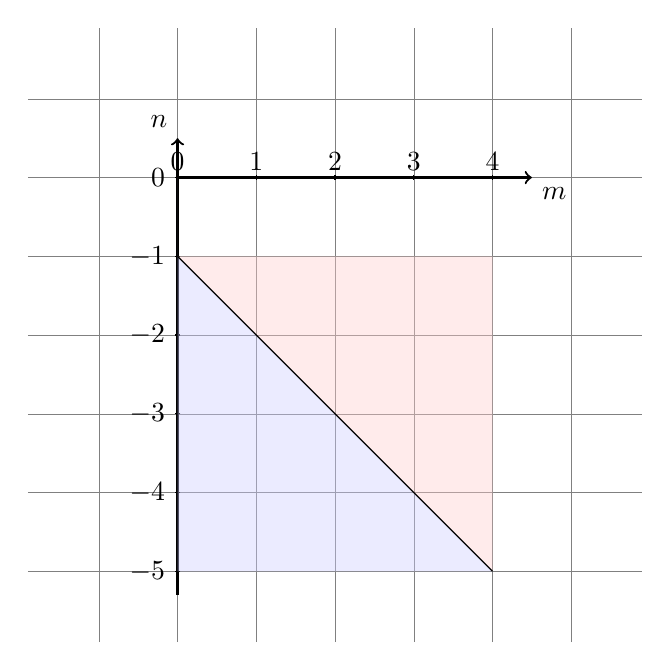
\begin{tikzpicture}
    \draw[step=1cm,gray,very thin] (-1.9,1.9) grid (5.9,-5.9);
    \draw[thick,->] (0,0) -- (4.5,0) node[anchor=north west] {\( m \)};
    \draw[thick,->] (0,-5.3) -- (0,0.5) node[anchor=south east] {\( n \)};
    \foreach \x in {0,1,2,3,4}
    \draw (\x cm,1pt) -- (\x cm,-1pt) node[anchor=south] {$\x$};
    \foreach \y in {0,-1,-2,-3,-4,-5}
    \draw (1pt,\y cm) -- (-1pt,\y cm) node[anchor=east] {$\y$};
    % \fill[blue!20, opacity=0.4] (-0.5, 0) -- (4, -4.5) -- (-0.5, -4.5) -- (-0.5, 0);
    % \fill[red!20, opacity=0.4] (0, -0.5) -- (4.5, -5) -- (4.5, -0.5) -- (0, -0.5);
    \fill[blue!20, opacity=0.4] (0, -1) -- (4, -5) -- (0, -5) -- (-0, 0);
    \fill[red!20, opacity=0.4] (0,-1) -- (4, -5) -- (4, -1) -- (1,-1);
    \draw (0, -1) -- (4, -5);
  \end{tikzpicture}

  \caption{TODO}
  \label{fig:nmregion}
\end{figure}

\begin{figure}[H]
  \centering
  \pgfplotsset{
    % colormap={X}{ gray(0cm)=(1); gray(1cm)=(0);},
    colormap={mycool}{ rgb255(0)=(255,0,255); rgb255(8)=(0,128,255); rgb255(10)=(255,255,255);},
  }
  \begin{tikzpicture}
    \begin{axis}[
      axis equal,
      xmin=0, xmax=12,
      ymin=-12, ymax=0,
      ]
      \addplot [
      matrix plot*,
      mesh/cols=12,
      point meta=explicit,
      ] table[x=m, y=n, meta=Contrib, col sep=comma] {data/tx0.csv};
    \end{axis}
  \end{tikzpicture}
  \begin{tikzpicture}
    \begin{axis}[
      axis equal,
      xmin=0, xmax=12,
      ymin=-12, ymax=0,
      ]
      \addplot [
      matrix plot*,
      mesh/cols=12,
      point meta=explicit,
      ] table[x=m, y=n, meta=Contrib, col sep=comma] {data/tx0.1.csv};
    \end{axis}
  \end{tikzpicture}
  \begin{tikzpicture}
    \begin{axis}[
      axis equal,
      xmin=0, xmax=12,
      ymin=-12, ymax=0,
      colorbar
      ]
      \addplot [
      matrix plot*,
      mesh/cols=12,
      point meta=explicit,
      ] table[x=m, y=n, meta=Contrib, col sep=comma] {data/tx0.4.csv};
    \end{axis}
  \end{tikzpicture}
  \caption{TODO}
\end{figure}

\subsection{Tilt parallell to the magnetic field}
We consider here a tilt parallel to the magnetic field, \( \vec{t} \parallel \vec{B} \). We will consider only the canonical part of the energy-momentum tensor, and not the full symmetrized form, as described \citeauthor{vanderwurffMagnetovorticalThermoelectricTransport2019} \cite{vanderwurffMagnetovorticalThermoelectricTransport2019}.
\begin{equation}
  \label{eq:94}
  T^{\mu 0} = \frac{i}{2}
  [
  \partial_j \bar{\psi} \Gamma ^j \gamma ^0 \Gamma ^{\mu } \psi - \bar{\psi} \Gamma ^{\mu } \gamma ^0 \Gamma ^j \partial _j \psi
  ],
\end{equation}
where \( \Gamma ^{\mu } = \gamma ^{\mu } + \gamma ^0 t^{\mu } \) with \( t^{\mu } = (0, \vec{t}) \) when inversion symmetry is broken and \( \Gamma ^{\mu }= \gamma ^{\mu } = \gamma ^0 \gamma ^5 t^{\mu } \) in the inversion symmetric case.

We have, with \( \vec{t}^{\chi } = \vec{t} \) in the inversion symmetric case, and \( \vec{t}^{\chi } = \vec{t} \) in the symmetry broken case.
The expression is exactly the same as for the untilted case, only with different energies.
The dimensionless quantities are
\begin{equation}
  \label{eq:95}
  \epsilon_{\kappa m s} =
  \begin{cases}
    t_z^{\chi } \kappa + \sign{m} \sqrt{M + \kappa ^2} & m \neq 0\\
    (t_z^{\chi } - s) \kappa & m = 0
  \end{cases}.
\end{equation}
The normalization factor \( \alpha _{\vec{k} m s} \) is, expressed in dimensionless quantities,
\begin{equation}
  \label{eq:96}
  \alpha _{\kappa m s} =
  -\sqrt{\frac{M}{(\epsilon_{\kappa  m s} - t_{z}^{\chi })s - \kappa }}.
\end{equation}
The integrand is
\begin{equation}
  \label{eq:97}
  \sum\limits_{mn}^{}
  (\epsilon_{\kappa m s} + \epsilon_{\kappa n s}) (\alpha_{\kappa n s}^2 \delta _{N, M+1}- \alpha_{\kappa m s}^2 \delta_{M, N+1}).
\end{equation}
As described above, the contributions from the \( \alpha _{\kappa n s}^2  \) and \( \alpha _{\kappa m s}^2 \) terms are identical, and we may simply take
\begin{equation}
  \label{eq:98}
  \sum\limits_{\underset{N=M+1}{mn}}^{}
  (\epsilon_{\kappa m s} + \epsilon_{\kappa n s}) \alpha_{\kappa n s}^2.
\end{equation}
For Type-I semimetals, the sign energy of state \( m \neq 0 \) is given by the sign of \( m \) itself.
For \( m = 0 \) the sign of the energy is given by \( -s \sign{\kappa } \).
Due to this, the sum is restricted to \( n=M+1, m=-M \) and \( n=-M-1, m=M \).
In the case of Type-II, however, the situation is not so simple.
The energy bands cross the Fermi surface, and we must also include in our sum overlap between states of the same sign, i.e. \( n=M+1, m=M \) and \( n=-M-1, m=-M \), which is non-zero for certain intervals of \( \kappa  \).
\todo{Include a figure}


\section{Notes}
\subsection{Spin states for Dirac cone}
See mathematica file.

Consider a simple Dirac cone Hamiltonian \(H_{D} = s v_{F} \vec{\sigma} \vec{p}\), with \(s\) denoting the chirality of the cone.
The eigenvalues of the system is of course \(E = \pm v_{F} k, \quad k=|\vec{k}|\).
We want to find the eigenstates of this system.
Assume plane wave state, and some arbitrary linear combination of spin up and spin down,
\[
  \psi _{\pm} = e^{i \vec{k} \vec{r}} \alpha
  \begin{pmatrix}
    1\\
    b
  \end{pmatrix},
\]
where \(\alpha \) is some normalization.
Solving the time independent Schrodinger equation
\[
H \psi = E \psi,
\]
we may solve for \(b\), which gives
\begin{equation}
  \label{eq:99}
  b = -\frac{k_{z} \pm k}{k_{x} - i k_{y}}.
\end{equation}
Requiring normalization of the state \(\braket{\psi | \psi } = 1\) gives the normalization
\[
|\alpha |^2 = \frac{1}{1 + |b|^2}.
\]

Having found the states, we find the spin expectation value
\begin{equation}
  \label{eq:100}
  \vec{S} = \braket{\psi | \hat{S} | \psi },
\end{equation}
where \(\vec{S}\) is the spin expectation value and \(\hat{S} = \frac{\vec{\sigma}}{2} \) is the spin operator, where \(\hbar \) was set to 1.
Simply evaluating Eq. \eqref{eq:100}, yields
\begin{equation}
  \label{eq:101}
  \vec{S} = \pm \frac{\vec{k}}{2 k}.
\end{equation}

The spin structure is that of a hedgehog.

\begin{figure}[ht]
  \centering
  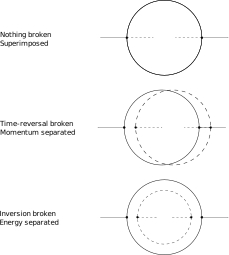
\includegraphics[width=0.75\textwidth]{figures/spinStructureWeyl}
  \caption{\label{fig:spinStructure} }
\end{figure}



\subsection{Symmetries}
In order to separate weyl cones in momentum, we introduce a pseuod spin degree of freedom, making the system 4x4.
We may then get solutions with the cones separated in momentum (or energy).
We may also ask what heppens if we try to separate tilted cones?

Firstly, in the most intuitive way to extend the 2x2 tilted cones to 4x4, we get that the cones tilt opposite direction, thus not superimposed even before separating in momentum.
They are after that simple to separate in momentum.
We might wonder if it makes sense to do it in this way.

The lattice model of the energy dispersion to explain tilted cones gives two cones separated in momentum, and tilting corresponds to ``bending'' the dispersion curves between them.
Maybe we therefore always have cones separated in momentum, and thus tilting superimposed does not make sense?
All depends on the origin of the tilt I believe.
Also, we must not confuse the global dispersion relation, to the Dirac cones which are expansions around the nodes.

Key to understand how spin behaves in all of this, and also maybe the symmetries.

To properly investigate the symmetry properties of the system, we must consider the 4x4, not 2x2 Hamiltonians.
While the 2x2 system does a goood job at describing a single cone, much important phsycis is lost when reducing the 4x4 Hamiltonian.
For example, the requirement that the total Berry curvature over the entire Briolluine zone is zero is not met for the 2x2 Hamiltonian, as it describes only one cone of a certain chirality.
The 4x4, however, includes two cones, which may in general be superimposed, thus conserving the total zero-divergence of the Berry curvature.
As a matter of fact, the inclusion of both cones is important also for symmetry considerations.

Let
\[
  H = v_{F} \tau _{x} \otimes \vec{\sigma} \vec{k},
\]
where \(\tau \) is some pseudo spin degree of freedom, transforming like \(\vec{r}\) under parity in time reversal.
This system describes two superimposed cones at the origin, with opposite chirality.
The effect of parity \(\mathcal{P}\) and time reversal \(\mathcal{T}\) is
\begin{table}[h]
  \centering
  \begin{tabular}{lcc}
    & \(\mathcal{P}\) & \(\mathcal{T}\)\\
    \hline
    \(\tau \) & - & +\\
    \(\sigma \) & + & -\\
    \(k\) & - & -
  \end{tabular}
\end{table}
\begin{equation}
  \label{eq:102}
  \begin{aligned}
    \mathcal{P} \tau \mathcal{P}^{\dagger} &= -\tau, & \mathcal{T} \tau \mathcal{T}^{\dagger} &= +\tau\\
    \mathcal{P} \sigma  \mathcal{P}^{\dagger} &= + \sigma,  & \mathcal{T} \sigma  \mathcal{T}^{\dagger} &= -\sigma \\
    \mathcal{P} k \mathcal{P}^{\dagger} &= -k, & \mathcal{T} k \mathcal{T}^{\dagger} &= -k
  \end{aligned}
\end{equation}
Obviously then, the Hamiltonian is both time reversal and parity invariant, as \(\mathcal{P} \mathcal{P}^{\dagger} = \mathcal{T} \mathcal{T}^{\dagger} = 1\).

A tilt term \(\tau _{x} \otimes \mathcal{I} \vec{\omega} _{0} \vec{k}\) breaks time reversal invariance, while maintaining parity invariance.
This is due to the two cones of opposite chirality tilting in opposite directions.

\begin{figure}[h]
  \centering
  \begin{tikzpicture}
    \draw[->] (-4, 0) -- (4, 0) node[right] {\(k\)};
    \draw[->] (0, 0) -- (0, 4) node[right] {\(E\)};

    % vf = 1, v0 = 0.8
    \draw[blue] (-3.5, 0.7) -- (0, 0) -- (2, 3.6) node[right] {\(\ket{\uparrow}\)} coordinate[pos=0.7] (a);
    \draw[red] (3.5, 0.7) node[right] {\(\ket{\downarrow }\)} -- (0, 0) -- (-2, 3.6)
    coordinate[pos=0.7] (b);

    \draw[->] (a) -- ++(1, 0);
    \draw[->] (b) -- ++(1, 0);
  \end{tikzpicture}
  \caption{Time reversal breaking in tilted system.
    Cross section in the tilt direction shown, with blue showing one cone and red the other.
    Black arrows indicate spin direction, which for \(\ket{\uparrow {}}\) is proporitional to  \(k\) while for \(\ket{\downarrow {}}\) is proportional to \( -k \).
  }
\end{figure}

The unperturbed Dirac Hamiltonian is Lorentz invariant, given that we consider an ``effective speed of light'', namely the Fermi velocity, instead of the actual speed of light \( c \).
Specifically, Lorentz invariance means invariance under the \emph{Lorentz group}.
The Lorentz group is the \( O(1,3) \) Lie group that conserves
\[
x_{\mu } x^{\mu } = t^2 - x^2 - y^2 - z^2,
\]
i.e. all isometries of Minkowski space.
More specifically, the group consists of all 3D rotations, \( O(3) \), and all \emph{boosts}.
A boost is a hyperbolic rotation from a spactial dimension to the temporal dimension.
If we now direct our focus at the Hamiltonian of the Dirac cone
\[
H = \pm v_{F} \vec{\sigma} \vec{p},
\]
we may easily show the Lorentz invariance of the system.
The time independent Schrodinger equation is
\begin{equation}
  \label{eq:103}
  H \ket{\psi } = E \ket{\psi } \implies (H^2 - E^2) \ket{\psi } = 0.
\end{equation}
As
\[
p^{\mu } = \left(\frac{E}{c}, \vec{p}\right),
\]
the operator in Eq. \eqref{eq:103} is nothing more than
\todo{ Make clear the matrix strucute here. There is an implicit identity matrix of size 2 }
\begin{equation}
  \label{eq:104}
  H^2-E^2 = v_{F}^2 \vec{p}^2 - c^2 \left(p^0\right)^2 ,
\end{equation}
where we used the anticommutation relation
\[
\{\sigma_{i}, \sigma_{j}\} =  2 \delta _{ij}
\]
of the Pauli matrices.
Using now the effective speed of light \( c=v_F \), Eq. \eqref{eq:104} is
\begin{equation}
  \label{eq:105}
  - v_F^2 p_{\mu } p^{\mu }.
\end{equation}
The invariance of \( x^{\mu} x_{\nu} \) is the very definition of the Lorentz group, and so is obviously Lorentz invariant.

Consider now a \emph{tilted} Dirac cone
\begin{equation}
  \label{eq:106}
  H = \pm v_F \vec{\sigma} \vec{p} + \omega_x k_x,
\end{equation}
where we, without loss of generality, chose the tilt to be in the \( x \)-direction.
By the same argumentation as above, the eigenequation
\[
  H \ket{\psi} = E\ket{\psi} \implies (H^2 - E^2)\ket{\psi} = 0
\]
leads to the equation
\begin{equation}
  \label{eq:116}
  -v_F^2 p^{\mu} p_{\mu} + \omega_{x} k_x (2 E - \omega_x k_x) = 0.
\end{equation}
This is \emph{not} invariant under a Lorentz transformation, as can be seen by, for example, a rotation around the \( z \)-axis.
\todo{Clean up p vs k}



\begin{figure}[h]
  \centering
  \begin{tikzpicture}
    \begin{groupplot}[
      group style={group size=1 by 4},
      cycle list name=linestyles,
      ymin=-3, ymax=3,
      xmin=-3, xmax=3,
      ]
      % \foreach \paramwpp in {0,0.2,0.5,1} {
      % \foreach \paramalpha in {1, 0.8, 0.5, 0.2} {
      \pgfplotsinvokeforeach{1,2,3,4} {
        \nextgroupplot
        \newcommand{\paramwpp}{0}
        \newcommand{\paramalpha}{#1}
        % \newcommand{\paramalpha}{0.5}
        % \begin{axis}[
        %   cycle list name=linestyles,
        %   ymin=-3, ymax=3,
        %   ]
        \addplot {(\paramwpp - \paramalpha)  * x};
        % \foreach \n in {1,2,3,4} {
        %   \addplot {
        %     \paramwpp * x + sqrt(2 * \n * \paramalpha ^ 3 + x^2 * \paramalpha ^ 2)
        %   };
        %   \pgfplotsset{cycle list shift=-1}
        %   \addplot {
        %     \paramwpp * x - sqrt(2 * \n * \paramalpha ^ 3 + x^2 * \paramalpha ^ 2)
        %   };
        % }

        \pgfplotsinvokeforeach{1,2,3,4} {
          \addplot {
            \paramwpp * x + sqrt(2 * ##1 * \paramalpha ^ 3 + x^2 * \paramalpha ^ 2)
          };
          \pgfplotsset{cycle list shift=-1}
          \addplot {
            \paramwpp * x - sqrt(2 * ##1 * \paramalpha ^ 3 + x^2 * \paramalpha ^ 2)
          };
        }
        % \end{axis}
      }
    \end{groupplot}
  \end{tikzpicture}

  \caption{}
\end{figure}
